\def\myversion{1.1}
\def\projectname{Kaiju Academy}

\documentclass[a4paper, 11pt]{scrreprt}
\usepackage{impl}  % Load Design Implementation document style
\setlist[itemize]{noitemsep,topsep=0pt,parsep=0pt,partopsep=0pt}
\usepackage{listings}
\usepackage{xcolor}
\usepackage{subcaption}
\usepackage{float}

\hypersetup{
    pdftitle={Design and Implementation for Kaiju Academy},
    pdfauthor={Group A2},
    pdfsubject={Technical Documentation},
    pdfkeywords={Design Implementation, Kaiju Academy, Software Engineering}
}

\lstdefinelanguage{Rust}{
  keywords={let, fn, mut, pub, self, struct, enum, match, if, else, return, where, impl, for, loop, while, break, continue, move, Box, Vec, Result, Option, Some, None, Ok, Err},
  keywordstyle=\bfseries\color{blue},
  identifierstyle=\color{black},
  sensitive=true,
  comment=[l]{//},
  morecomment=[s]{/*}{*/},
  commentstyle=\color{green!50!black},
  stringstyle=\color{red},
  morestring=[b]",
  morestring=[b]',
  basicstyle=\ttfamily\small,
  breaklines=true,
  showstringspaces=false,
  frame=single
}

\graphicspath{{./img/}}

\begin{document}

\pagenumbering{roman}

\begin{titlepage}
    \begin{flushright}
        \rule{\textwidth}{5pt}\vskip1cm
        \begin{bfseries}
            \Huge{DESIGN AND IMPLEMENTATION\\ FOR}\\
            \vspace{1.6cm}
            \projectname\\
            \vspace{1.6cm}
            \LARGE{Version \myversion}\\
            \vspace{1.6cm}
            Prepared by\\
            Group A2\\
            \Large{
                \begin{tabularx}{\textwidth}{l l >{\raggedleft\arraybackslash}X}
                    YU Ching Hei & 1155193237 & \href{mailto:chyu@link.cuhk.edu.hk}{chyu@link.cuhk.edu.hk}\\
                    Lei Hei Tung & 1155194969 & \href{mailto:1155194969@link.cuhk.edu.hk}{1155194969@link.cuhk.edu.hk}\\
                    Ankhbayar Enkhtaivan & 1155185142 & \href{mailto:1155185142@link.cuhk.edu.hk}{1155185142@link.cuhk.edu.hk}\\
                    Yum Ho Kan & 1155195234 & \href{mailto:1155195234@link.cuhk.edu.hk}{1155195234@link.cuhk.edu.hk}\\
                    Leung Chung Wang & 1155194650 & \href{mailto:1155194650@link.cuhk.edu.hk}{1155194650@link.cuhk.edu.hk}\\
                \end{tabularx}
            }\\
            \vspace{1.6cm}
            The Chinese University of Hong Kong\\
            Department of Computer Science and Engineering\\
            CSCI3100: Software Engineering\\
            \vspace{1.6cm}
            \today\\
        \end{bfseries}
    \end{flushright}
\end{titlepage}

\setuptoc{toc}{totoc}
\tableofcontents

\addchap{Document Revision History}
\begin{center}
    \begin{tabularx}{\textwidth}{>{\raggedright\arraybackslash}p{2cm}>{\raggedright\arraybackslash}p{3cm}>{\raggedright\arraybackslash}p{3cm}>{\raggedright\arraybackslash}X}
        \toprule
        Version & Revised By & Revision Date & Comments\\
        \midrule
        0.1 & Group A2 & 2025-02-27 & \begin{revisionitem}[Added:]
            \item Initial document structure
            \item Basic content outline
        \end{revisionitem}\\
        \midrule
        1.0 & Group A2 & 2025-03-11 & \begin{revisionitem}[Updated:]
            \item Final review and integration
        \end{revisionitem}\\
        \midrule
        1.1 & C. W. Leung & 2025-04-23 & \begin{revisionitem}[Updated:]
            \item Pruned and updated per requirements in meeting1.docx
        \end{revisionitem}\\
        \bottomrule
    \end{tabularx}
\end{center}

\clearpage
\pagenumbering{arabic}
\ofoot{Page \thepage\ of \pageref{LastPage}}

\chapter{Introduction}

Kaiju Academy is a \textbf{web-based e-learning platform} designed to make learning programming accessible and engaging. It combines modern Learning Management System (LMS) capabilities with interactive coding features, enabling users to learn at their own pace.

\section{Summary of Requirements}
Kaiju Academy includes:

\begin{itemize}
    \item \textbf{User Management \& Authentication:} Role-based access control for users (student), teachers (educator), and admins, with secure authentication and optional MFA.
    \item \textbf{Course Creation \& Management:} Tools for creating, updating, and organizing courses with videos, PDFs, quizzes, and coding assessments.
    \item \textbf{Interactive Learning:} Real-time code execution and automated grading via an online code editor.
    \item \textbf{Profile and Progress:} User and educator profiles, progress tracking, recommended and registered courses.
    \item \textbf{Monetization:} Course credit system for payment and buying credits to unlock courses.
\end{itemize}

\section{Quality Goals}
\begin{table}[htp]
    \centering
    \begin{tabularx}{\textwidth}{|l|X|}
        \hline
        \textbf{Goal} & \textbf{Description} \\
        \hline
        \textbf{Performance} & - Response time <2 seconds for 95\% of users. \newline - Code execution results in <5 seconds for 99\% of submissions. \\
        \hline
        \textbf{Scalability} & - Support 10,000 concurrent users. \newline - Horizontal scaling via AWS Lambda and SurrealDB sharding. \\
        \hline
        \textbf{Reliability} & - 99.9\% uptime with automatic failover. \newline - Recovery from failures within 5 minutes. \\
        \hline
        \textbf{Security} & - AES-256 encryption for data at rest. \newline - TLS 1.2+ for data in transit. \newline - Role-based permissions and MFA. \\
        \hline
    \end{tabularx}
    \caption{Quality Goals for Kaiju Academy}
\end{table}

\section{Stakeholders}
\begin{table}[htbp]\setlength{\abovecaptionskip}{0pt}
    \centering
    \begin{tabularx}{\textwidth}{|l|X|}
        \hline
        \textbf{Stakeholder} & \textbf{Role \& Responsibilities} \\
        \hline
        \textbf{Admin} & - Manage system health, user roles, and platform configurations. \newline - Enforce security policies. \\
        \hline
        \textbf{User (Student)} & - Enroll in courses, complete assessments, and track progress. \\
        \hline
        \textbf{Teacher (Educator)} & - Create and update course content. \newline - Grade submissions and provide feedback. \\
        \hline
    \end{tabularx}
    \caption{Stakeholders and Their Roles}
\end{table}

\subsection{Acknowledgments}
This document was prepared with the assistance of AI tools (e.g., ChatGPT 4.1) for drafting and review.

\chapter{System Architecture}

\section{Major Components}

\begin{description}
    \item[Frontend Application:] A React application providing the user interface across all devices.
    \item[Backend Services:] Rust-based AWS Lambda functions for service logic.
    \item[SurrealDB:] Primary database for persistent data.
    \item[AWS Services:] API Gateway, Lambda, Cognito (auth/MFA), S3 (media), CloudFront (CDN), Fargate (code execution).
\end{description}

\section{Component Relationships}
\begin{figure}[!htb]
    \centering
    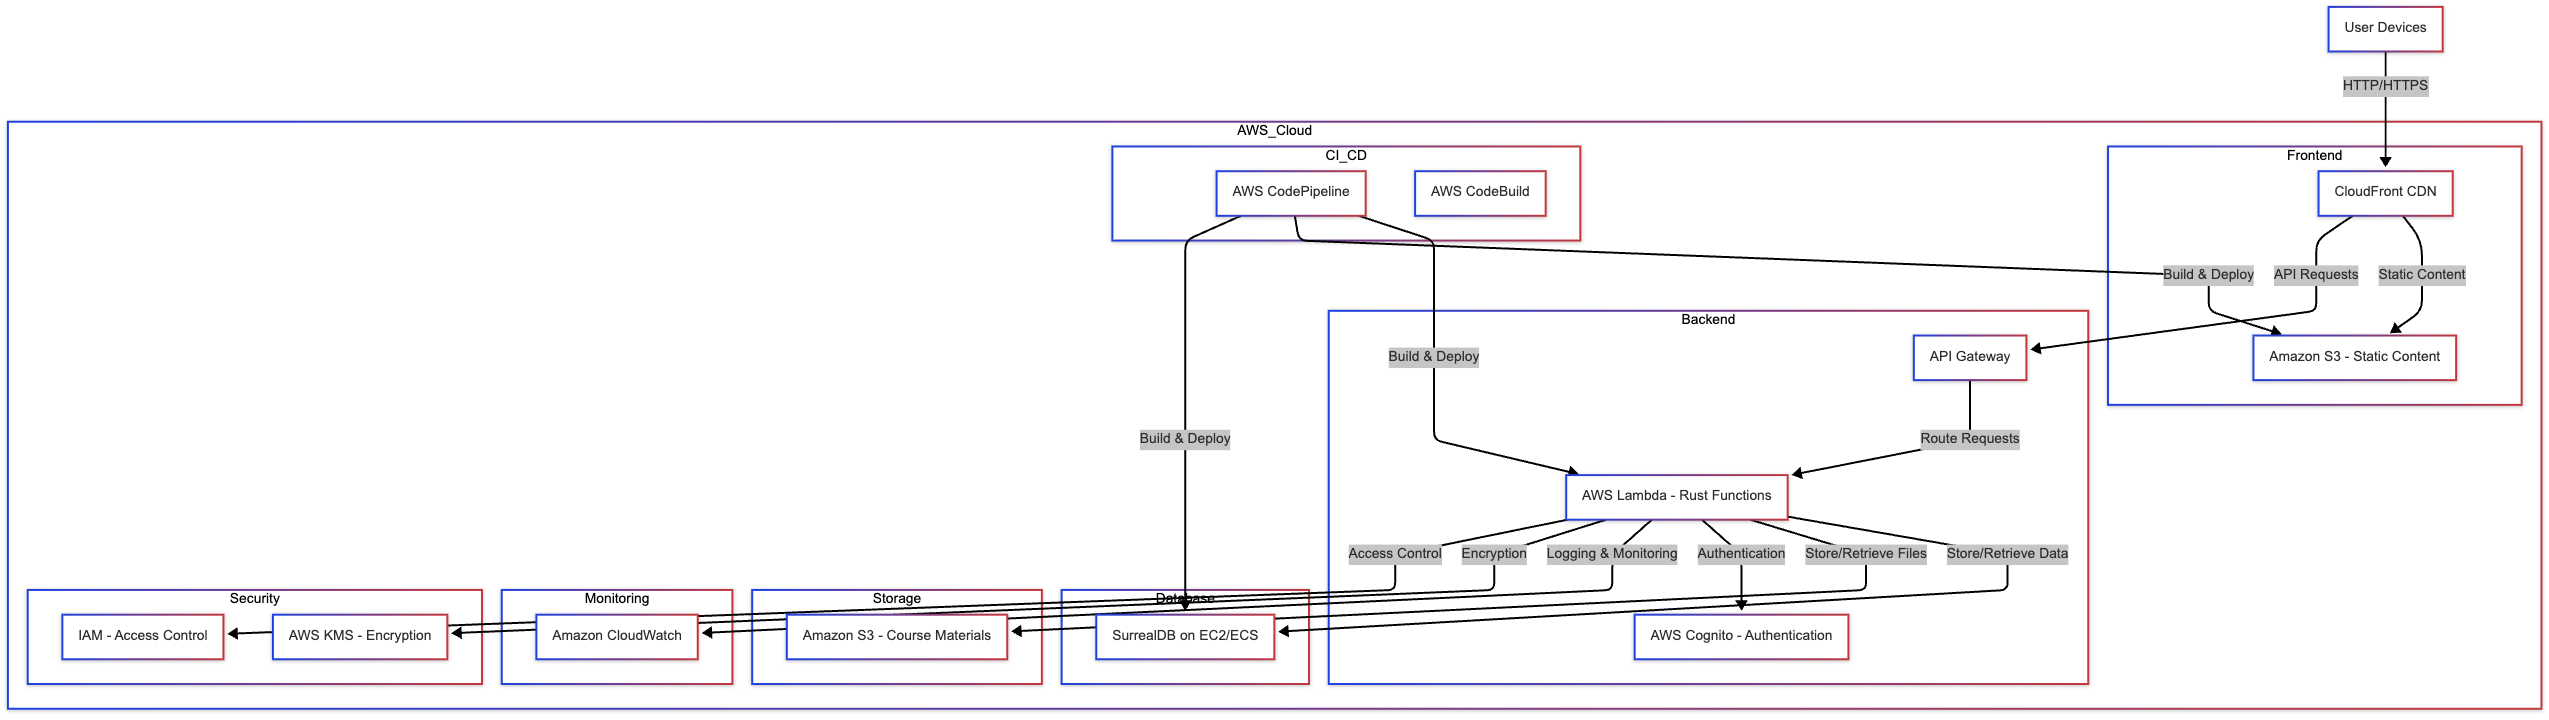
\includegraphics[width=0.5\textwidth]{serverless_deployment.png}
    \caption{AWS Serverless Deployment Architecture}
\end{figure}

\begin{itemize}
    \item Users access via browsers, routed through CloudFront CDN and API Gateway.
    \item Lambda functions handle business logic, SurrealDB stores data.
    \item Cognito manages authentication and optional MFA.
    \item S3 stores learning materials.
\end{itemize}

\section{Database}
SurrealDB's multi-model database supports course, user, credit/payment, progress, and assessment data.

\section{Security}
\begin{itemize}
    \item AWS-managed VPC and IAM boundaries.
    \item AES-256 encryption at rest, TLS 1.2+ in transit.
    \item JWT for stateless API authentication, MFA support via Cognito.
\end{itemize}

\section{User Authentication and Authorization}
\begin{itemize}
    \item Email/password registration and login, MFA if supported.
    \item JWT tokens for session management.
    \item Roles: user (student), teacher (educator), admin.
\end{itemize}

\section{Testability}
\begin{itemize}
    \item Automated unit and integration tests in Rust.
    \item CI/CD pipeline with test coverage enforcement.
\end{itemize}

\chapter{Data Models}

\section{Database Schema}
\begin{figure}[!ht]
    \centering
    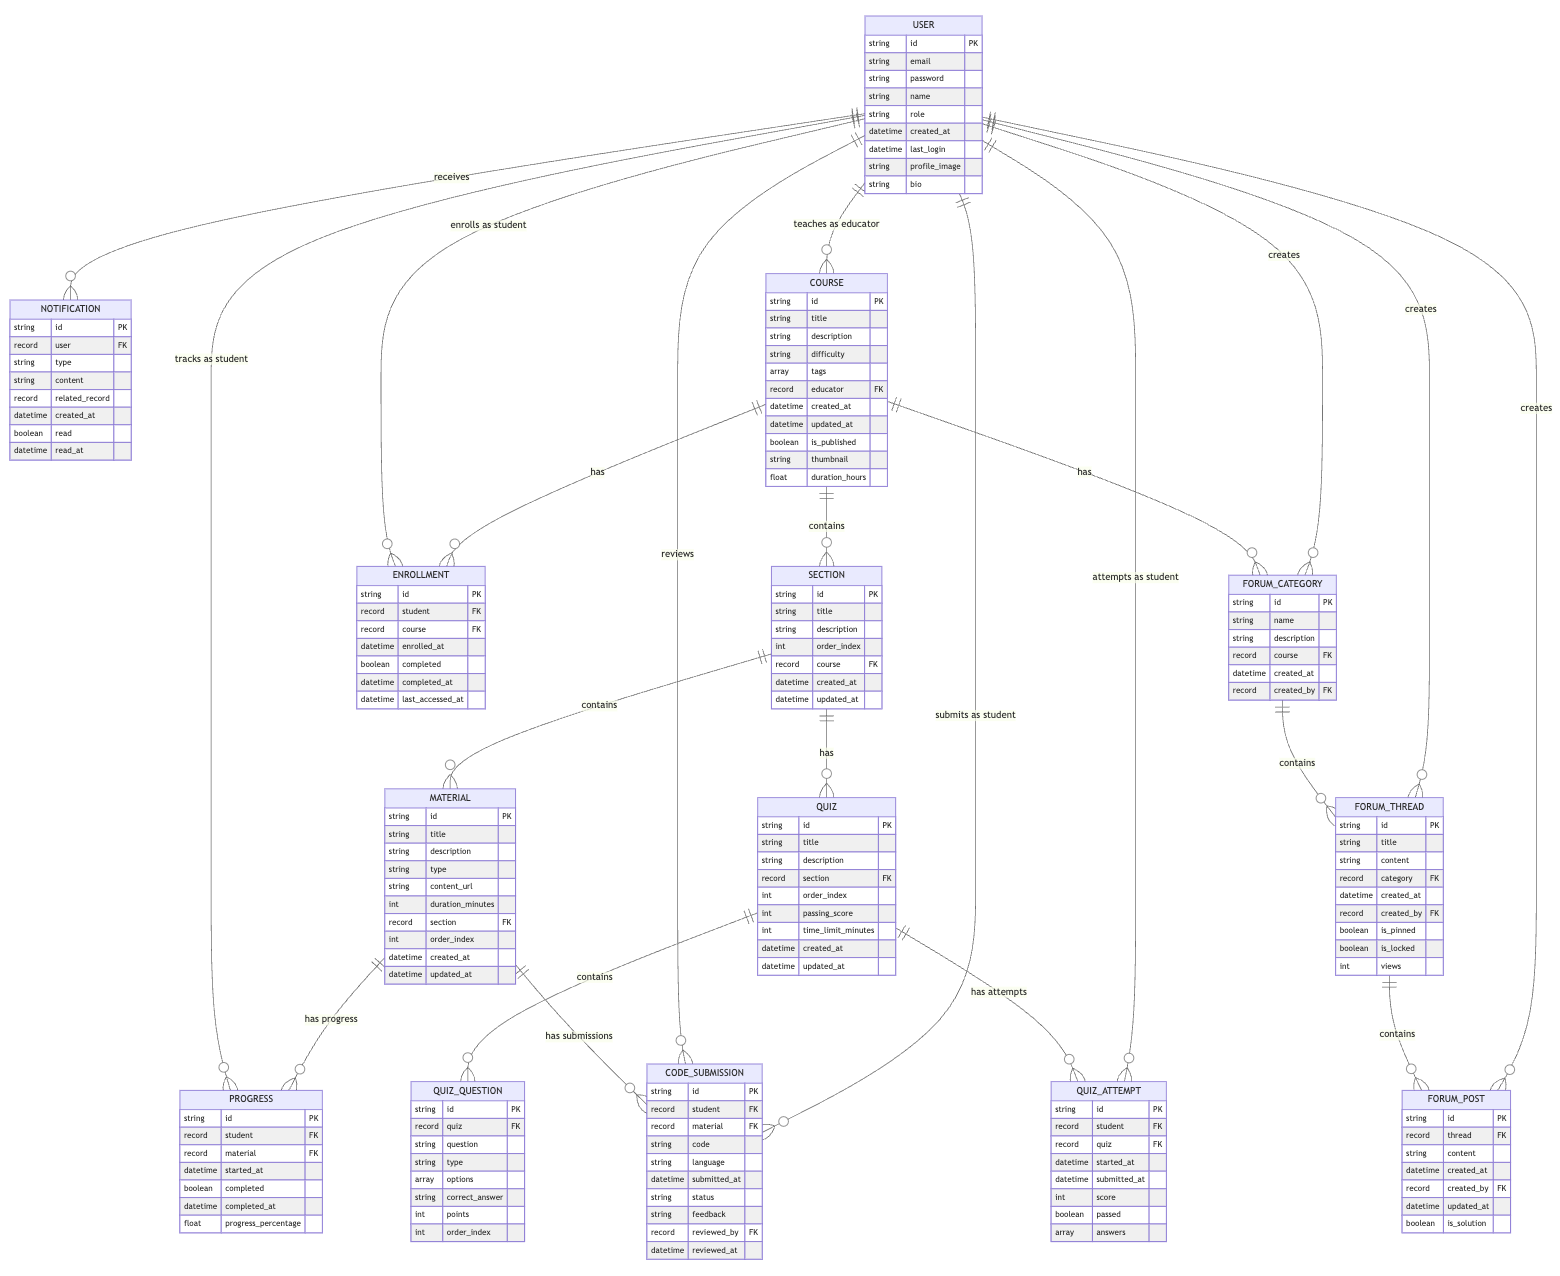
\includegraphics[width=\textwidth]{database_schema.png}
    \caption{Database Schema}
\end{figure}

\section{Request and Response Structure}
\begin{lstlisting}[language=Rust]
let response = ApiGatewayProxyResponse {
    status_code: 200,
    headers: std::collections::HashMap::new(),
    multi_value_headers: std::collections::HashMap::new(),
    body: Some(json!({ "message": "Hello from Kaiju Academy API!" }).to_string()),
    is_base64_encoded: Some(false),
};
Ok(response)
\end{lstlisting}

\section{Data Flow Sequence}
\begin{figure}[ht]
    \centering
    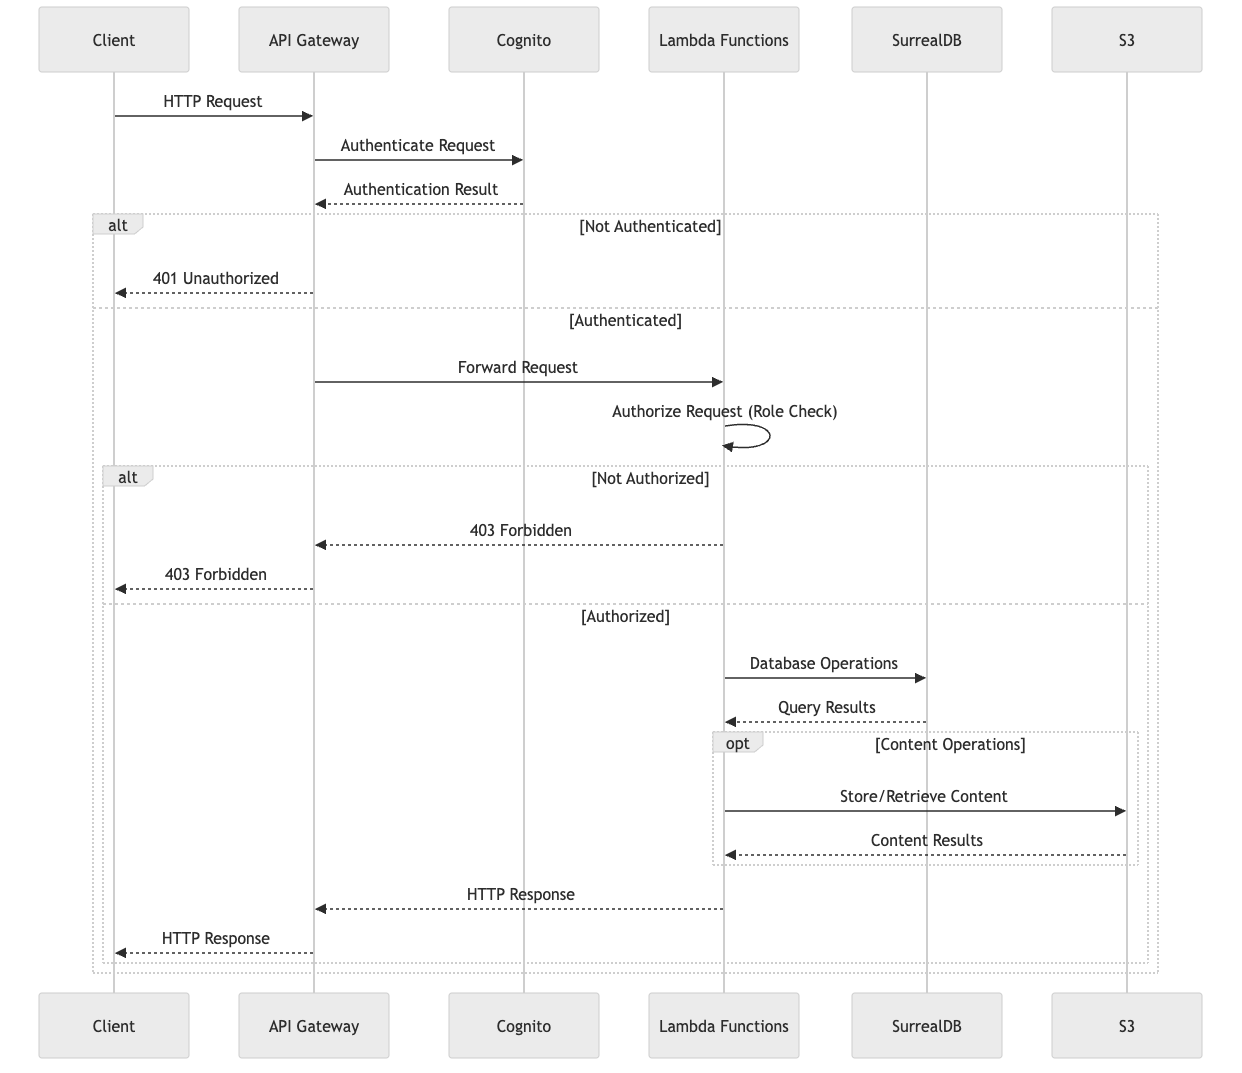
\includegraphics[width=\textwidth]{data_flow.png}
    \caption{Data Flow Sequence Diagram}
\end{figure}

\chapter{Interface Design}

\section{User Registration and Authentication}
\begin{figure}[!htb]
    \centering
    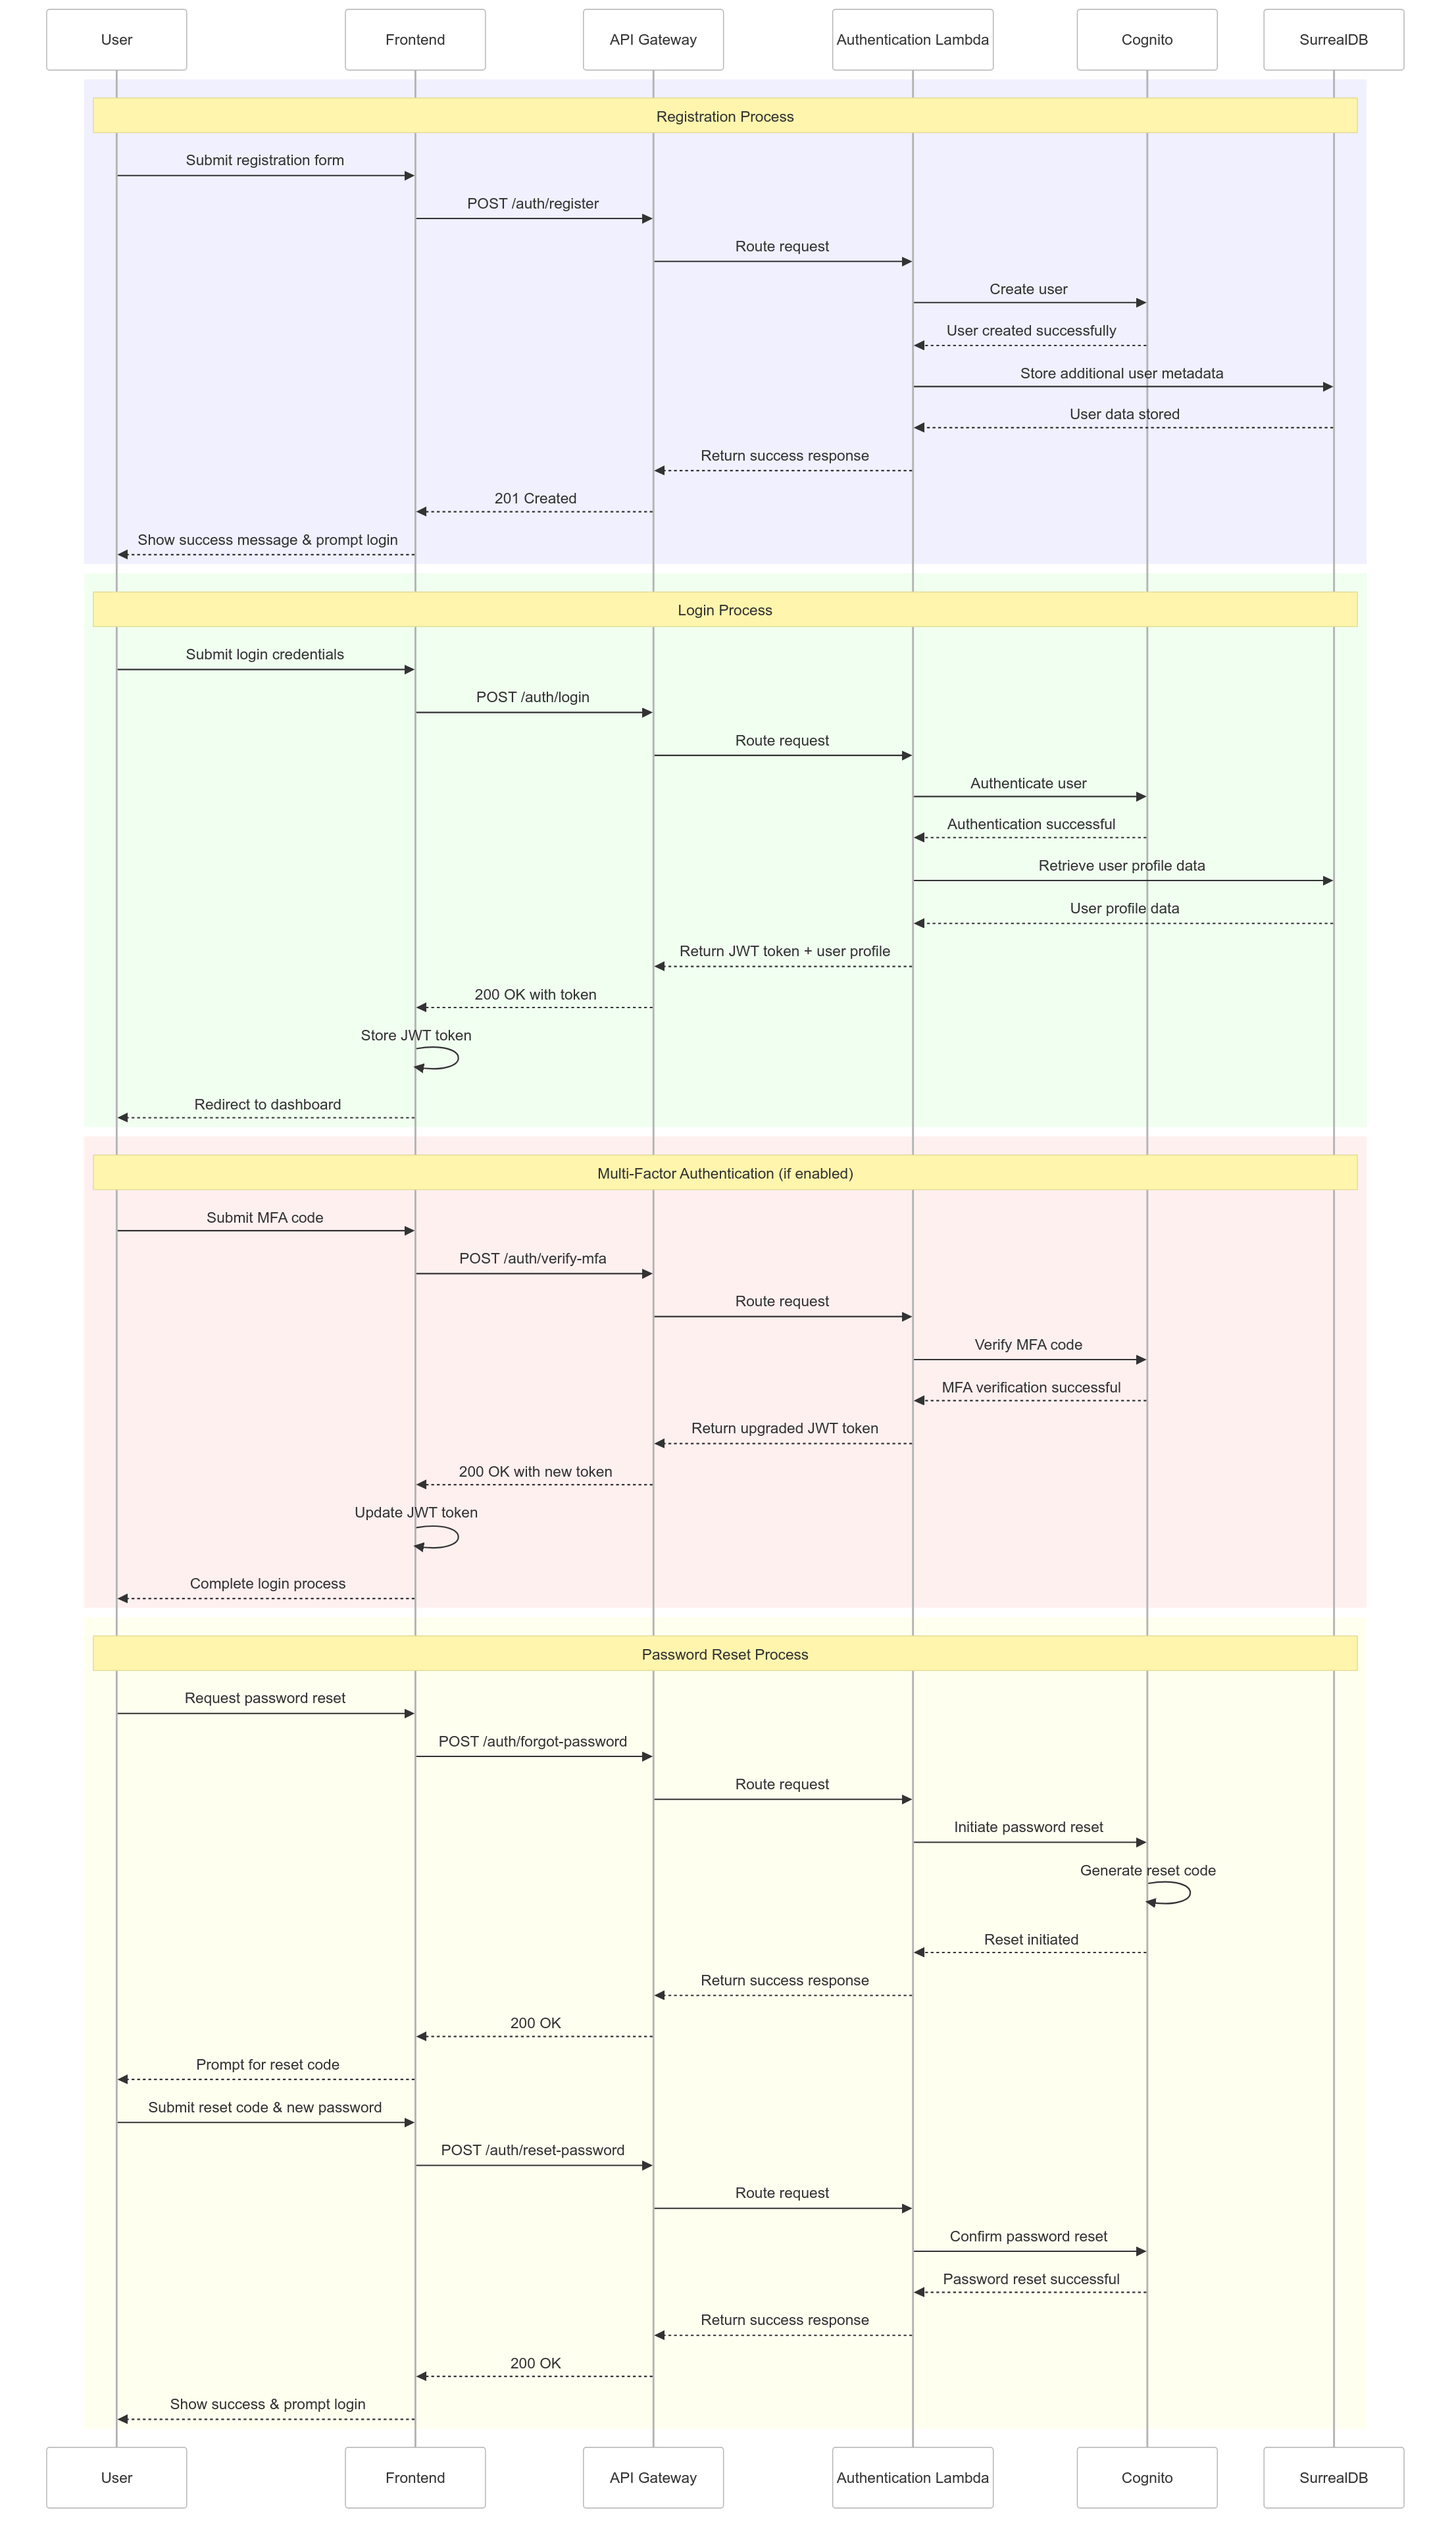
\includegraphics[height=0.7\textheight]{user_authentication.png}
    \caption{User Authentication Workflow}
\end{figure}
\begin{enumerate}
    \item User submits registration/login with optional MFA.
    \item API Gateway routes to Authentication Lambda.
    \item Lambda creates/validates user in Cognito and SurrealDB.
    \item JWT token returned for session.
\end{enumerate}

\subsection{Course Management}
\begin{figure}[!htb]
    \centering
    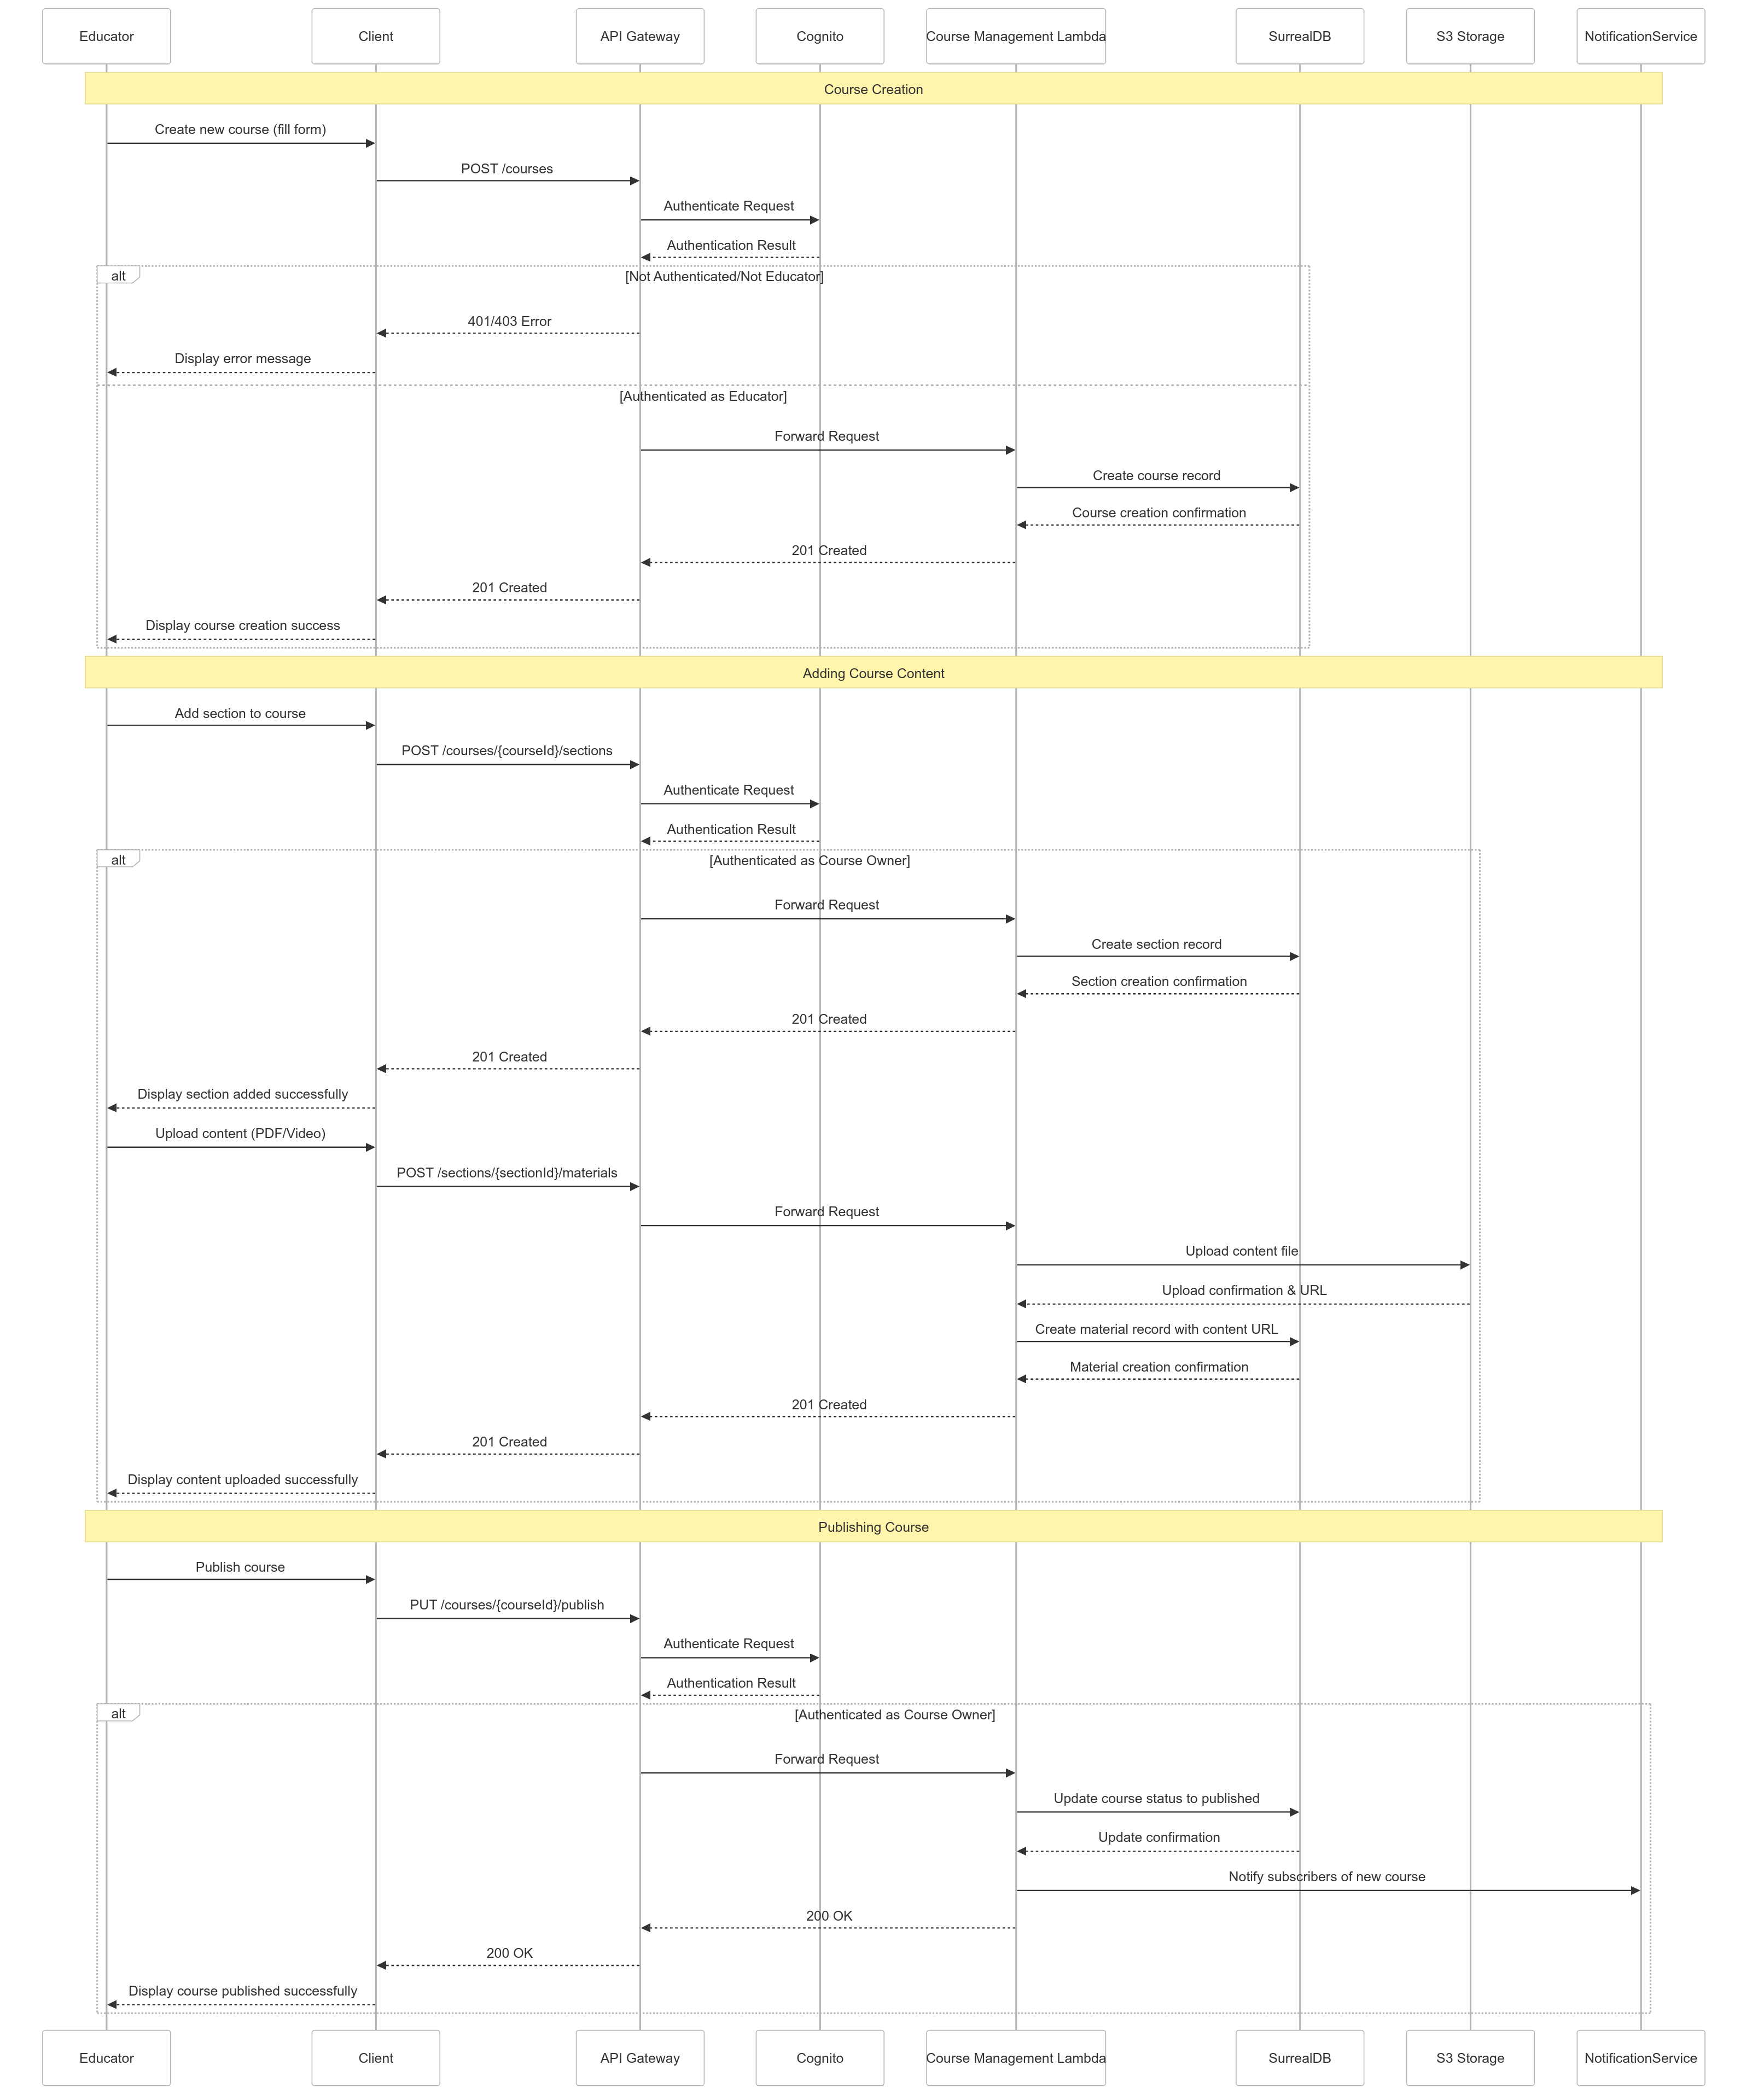
\includegraphics[height=0.75\textheight]{educator_managing_courses.png}
    \caption{Course Management Workflow}
\end{figure}
\begin{enumerate}
    \item Educator manages course structure and modules.
    \item Materials uploaded to S3.
    \item Changes stored in SurrealDB.
\end{enumerate}

\subsection{Course Access}
\begin{figure}[!htb]
    \centering
    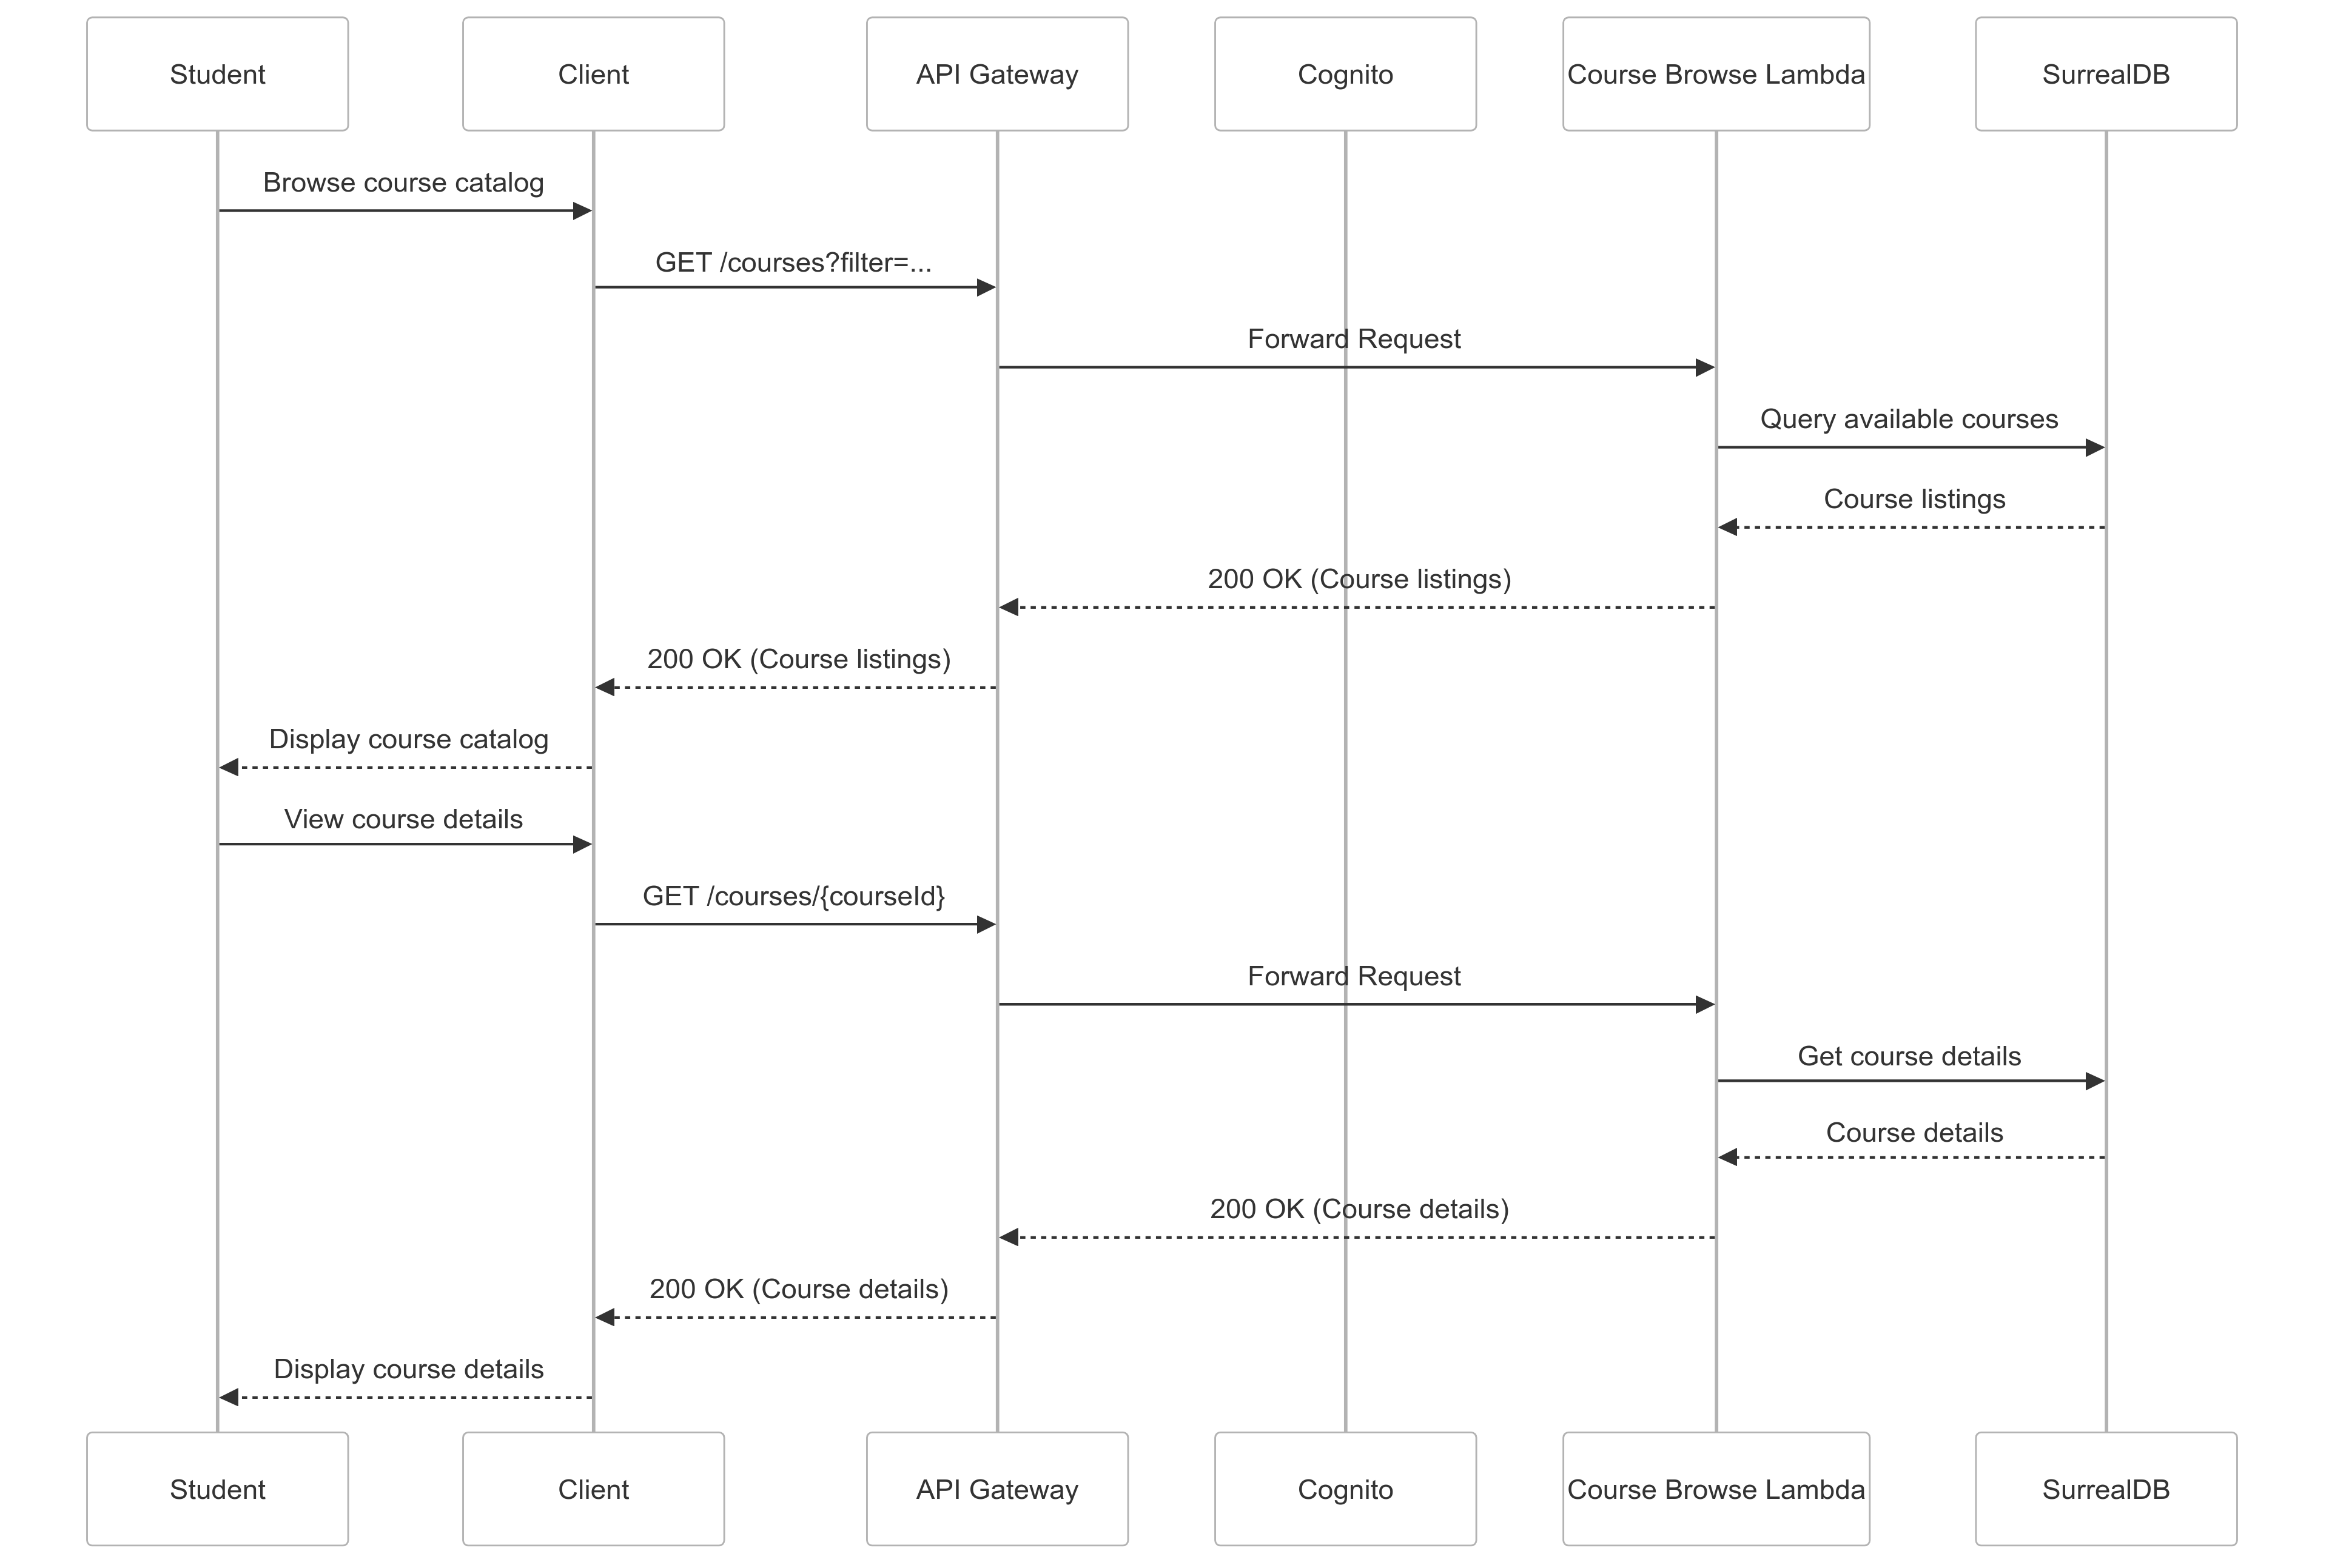
\includegraphics[height=0.4\textheight]{student_access_course.png}
    \caption{Course Access Workflow}
\end{figure}

\subsection{Code Assessment and Grading}
\noindent\textbf{Sample code assessment editor (simplified):}
\begin{lstlisting}[language=Rust]
// Code Assessment Editor (conceptual)
fn CodeEditor() {
    let code = "// Write your code here";
    fn run_code() {
        // send code to backend, display result
    }
    // Renders a textarea and Run button
}
\end{lstlisting}

\begin{figure}[!htb]
    \centering
    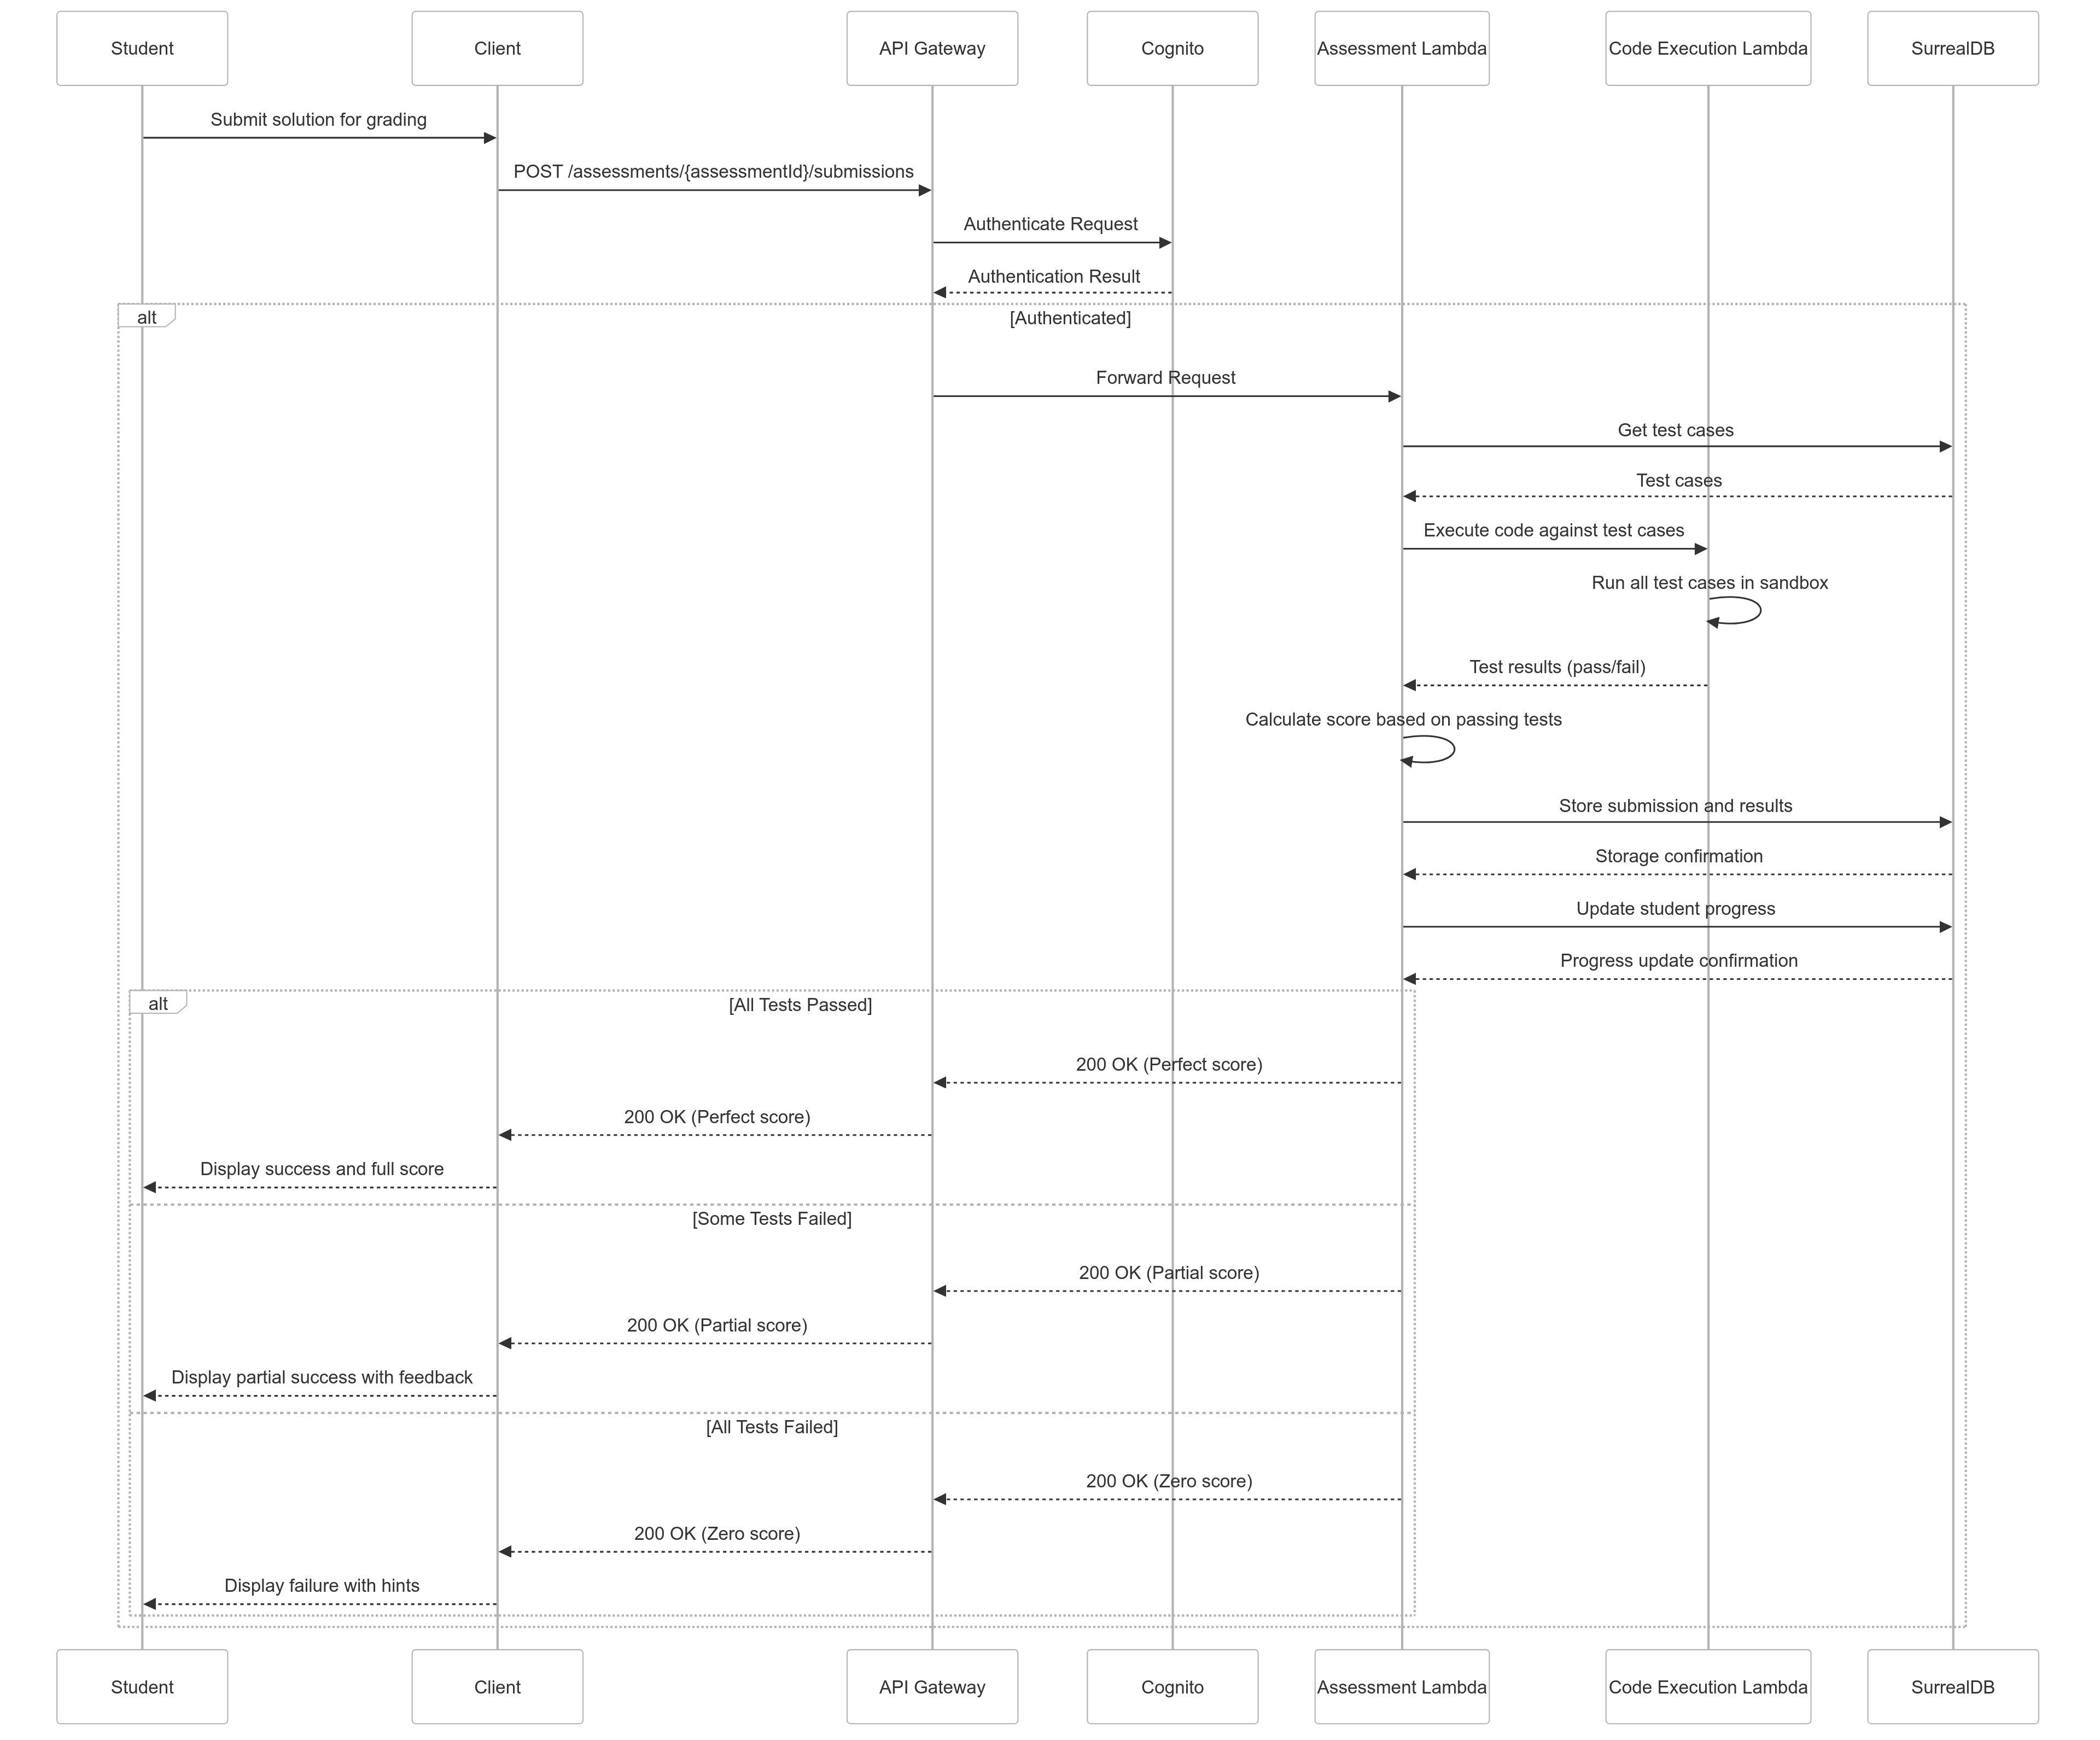
\includegraphics[height=0.4\textheight]{code_grade.png}
    \caption{Code Auto-grading Workflow}
\end{figure}

\section{Service Communication}
\begin{itemize}
    \item RESTful APIs with JSON payloads.
    \item Rate limiting per user/IP.
    \item Batch operations and pagination.
\end{itemize}

\section{Security Implementation}
\begin{itemize}
    \item Multi-factor Authentication (MFA) optional for all users.
    \item OAuth2 integration for social login.
    \item JWT for API authentication.
    \item AES-256 encryption for sensitive data.
\end{itemize}

\section{Exception Handling}
\subsection{Expected Exceptions}
\begin{itemize}
    \item Authentication errors (401)
    \item Authorization errors (403)
    \item Validation errors (400)
    \item Not found errors (404)
    \item Database errors (500)
    \item Internal server errors (500)
    \item External service errors (502)
    \item Rate limit errors (429)
\end{itemize}
\subsection{Error Handling Example}
\begin{lstlisting}[language=Rust]
impl From<AppError> for ApiGatewayProxyResponse {
    fn from(error: AppError) -> Self {
        let (status_code, error_type) = match &error {
            AppError::Authentication(_) => (401, "Authentication Error"),
            AppError::Authorization(_) => (403, "Authorization Error"),
            AppError::NotFound(_) => (404, "Not Found"),
            AppError::Validation(_) => (400, "Validation Error"),
            AppError::Database(_) => (500, "Database Error"),
            AppError::Internal(_) => (500, "Internal Server Error"),
            AppError::ExternalService(_) => (502, "External Service Error"),
            AppError::RateLimit(_) => (429, "Rate Limit Exceeded"),
        };
        // Response body omitted for brevity
        ApiGatewayProxyResponse { ... }
    }
}
\end{lstlisting}

\subsection{Credit Purchase and Payment Flow}

\textbf{Overview:}

Kaiju Academy uses a credit-based payment system. Users buy credits through an integrated payment gateway and spend credits to unlock/register for courses. This system decouples payment from course registration and supports flexible monetization.

\subsection{Credit Purchase and Course Enrollment Flow}

\begin{enumerate}
    \item User navigates to the ``Buy Credits'' page from the profile or course page.
    \item User selects a credit package (e.g., 100 credits, 200 credits).
    \item User is redirected to a third-party payment gateway (e.g., Stripe) to complete the transaction.
    \item Upon successful payment, the backend updates the user's credit balance.
    \item User can now browse courses; when enrolling in a paid course, the platform checks credit balance:
        \begin{itemize}
            \item If sufficient, deducts credits and confirms registration.
            \item If insufficient, prompts the user to buy more credits.
        \end{itemize}
    \item All transactions are logged for auditing and user transparency.
\end{enumerate}

\textbf{Security Note:} All payment processing is handled via a PCI-compliant gateway. No sensitive payment data is stored on Kaiju Academy servers.

\subsection{Credit Purchase and Enrollment Logic (Mermaid Diagram)}

% If you export this Mermaid diagram as SVG or PNG, include with:
\begin{figure}[ht]
    \centering
    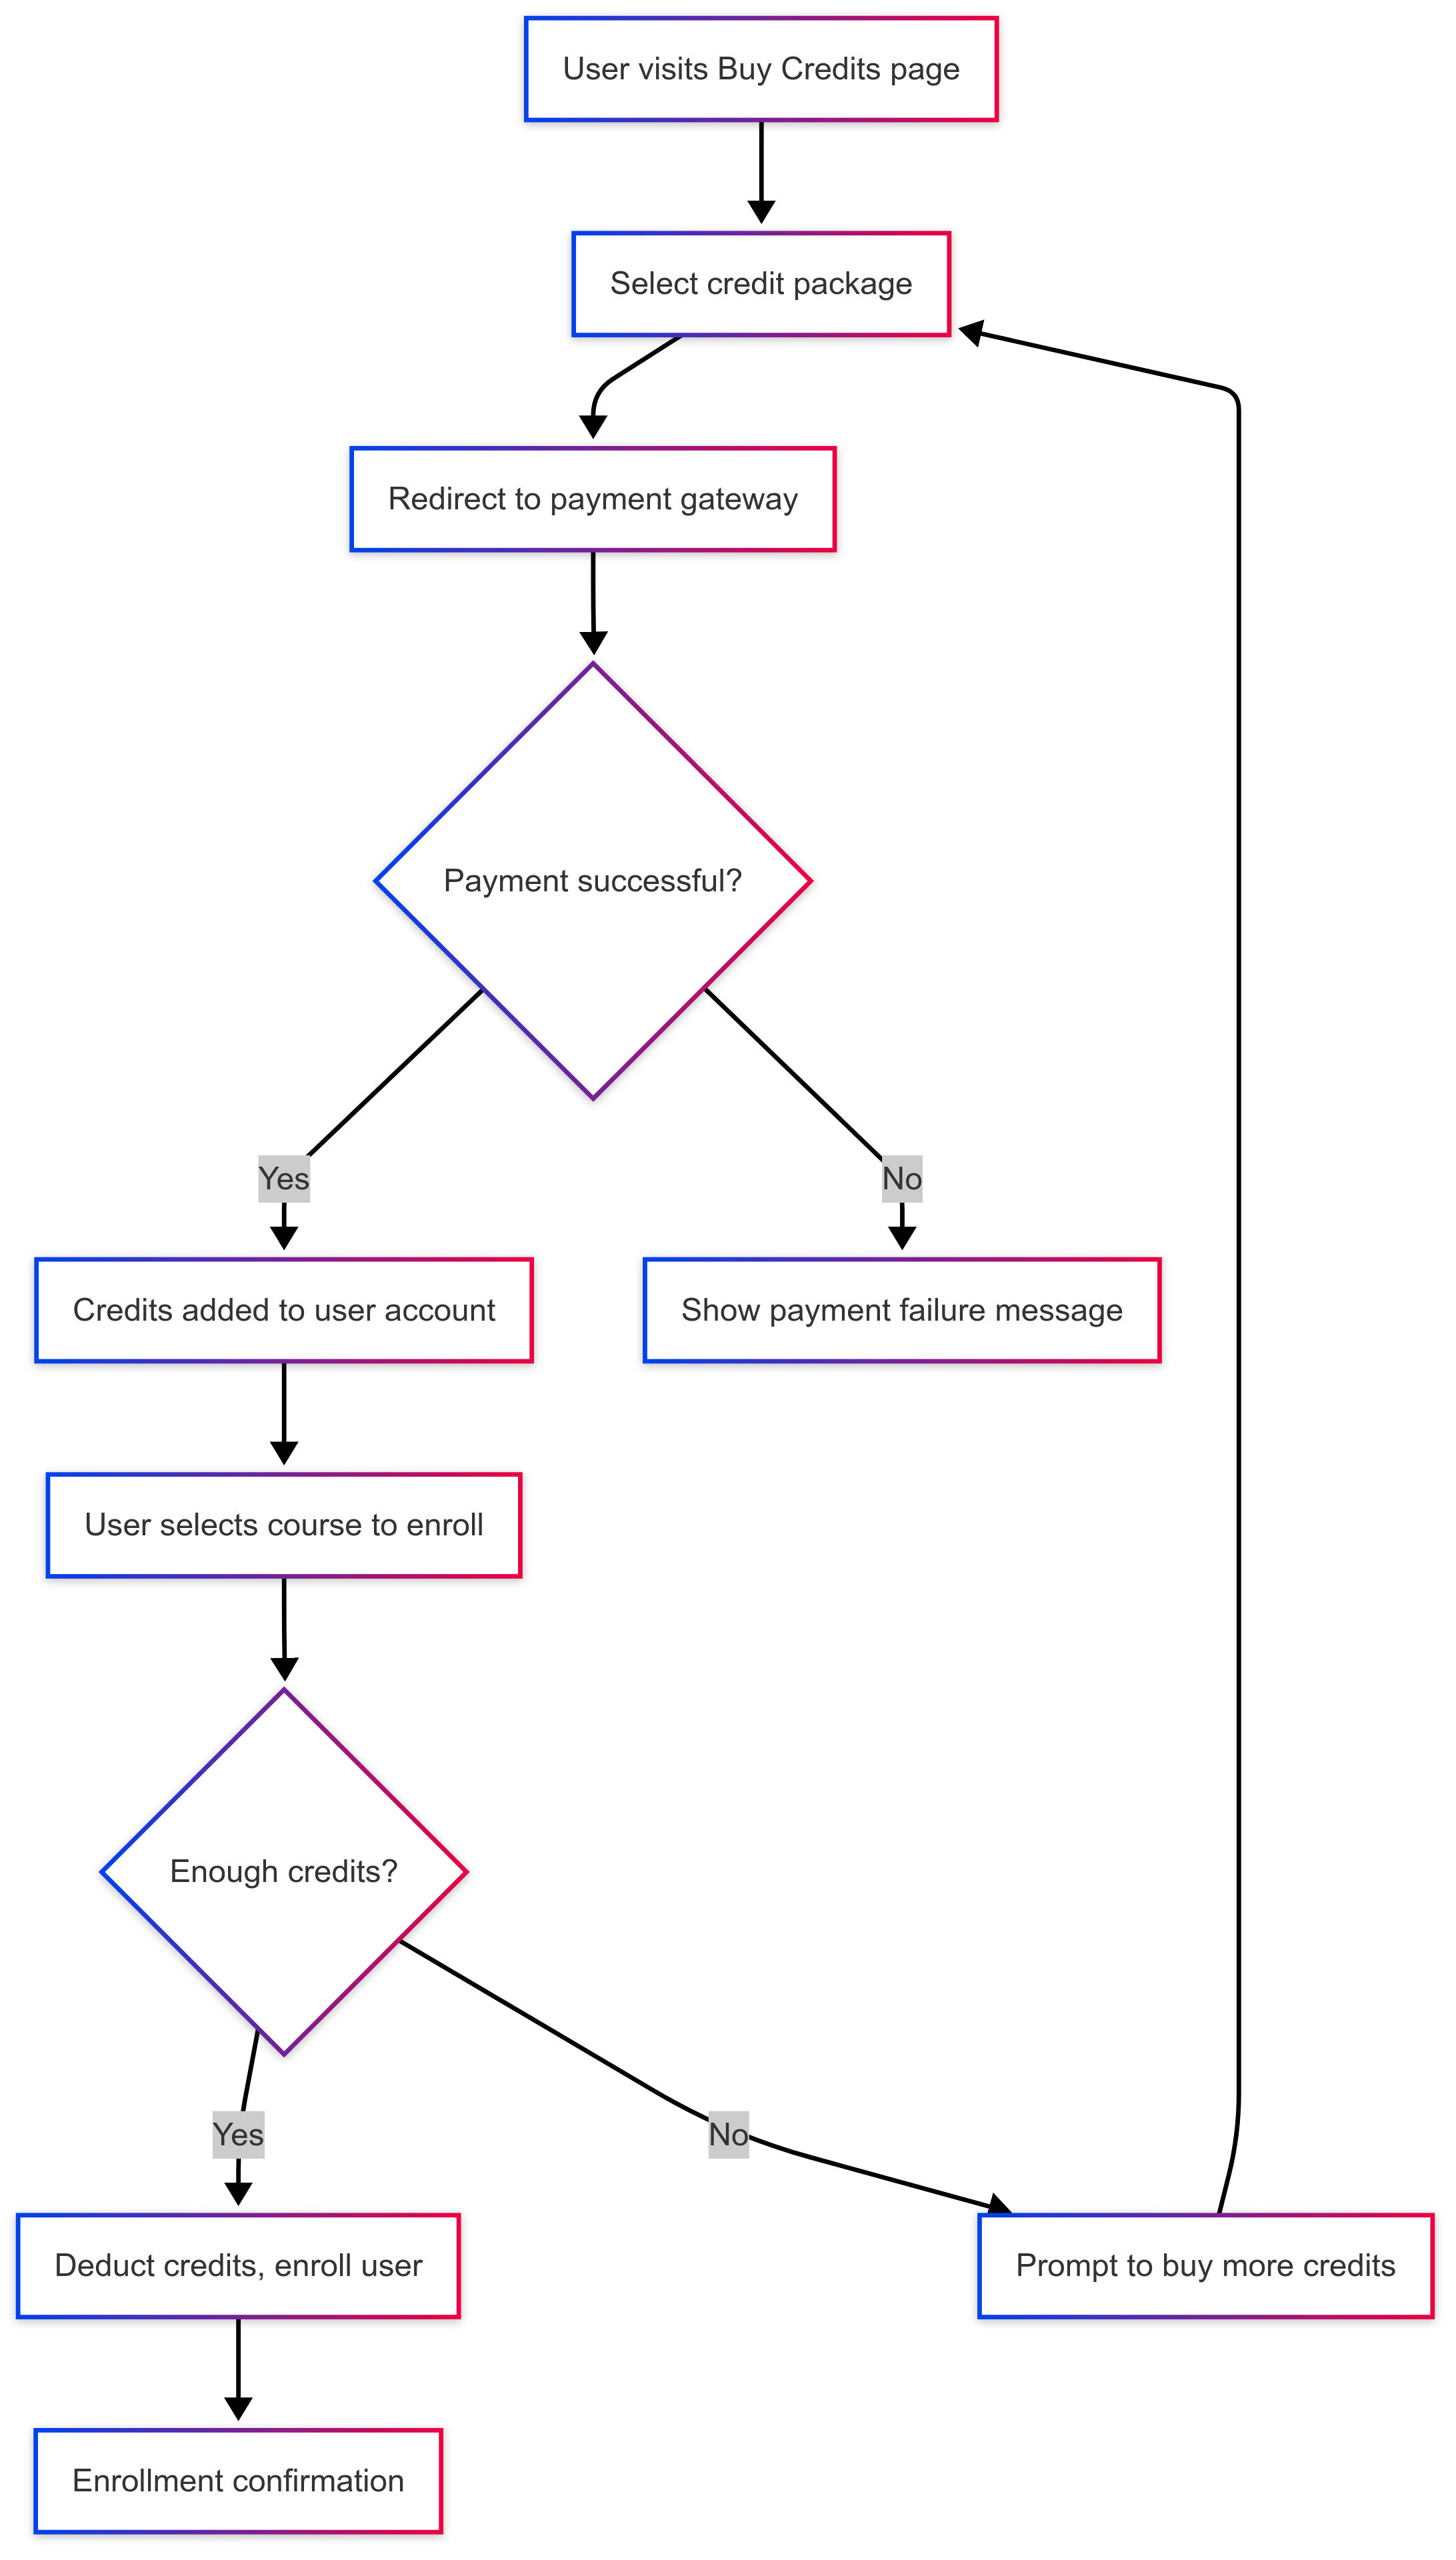
\includegraphics[width=0.4\textwidth]{img/credit_purchase_flow.png}
    \caption{Credit Purchase and Course Enrollment Flow}
\end{figure}

\section{Licence Key Verification}

\textbf{Overview:} \\
Upon first login or before accessing any main features, users must enter a valid licence key. The backend validates the key against a list (hardcoded or stored in the database). If the key is valid, access is granted; otherwise, the user is denied access and prompted again.

\begin{enumerate}
    \item After successful login, the user is prompted for a licence key.
    \item The entered key is sent to the backend for validation.
    \item If valid, the session is marked as “licenced” and the user proceeds.
    \item If invalid, an error message is displayed and access is denied.
\end{enumerate}

\textbf{Minimal Implementation Note:} \\
If time is limited, licence management may be implemented as a stub or described as future work, but the design must be documented.

\textbf{Security Note:} \\
Licence keys must not be predictable and should be stored securely.


\chapter{Component Design}

\section{Frontend Components}

\subsection{Navbar Component}
\begin{itemize}
    \item \textbf{Intention:} Provides navigation links and user profile access.
    \item \textbf{Input:} User interactions (clicks), authentication state.
    \item \textbf{Output:} Navigation actions, profile dropdown.
\end{itemize}

% Dashboard and forum-related components removed

\subsection{Code Editor Component}
\begin{itemize}
    \item \textbf{Intention:} Provides syntax highlighting, code execution, and result display.
    \item \textbf{Input:} User code, language, test cases.
    \item \textbf{Output:} Code submission to backend, execution result.
\end{itemize}

\section{Backend Components}

\subsection{Authentication Service}
\begin{itemize}
    \item \textbf{Intention:} Registration, login, MFA, token management.
    \item \textbf{Input:} Credentials, MFA codes.
    \item \textbf{Output:} JWT tokens, authentication status, error messages.
\end{itemize}

\subsection{Course Management Service}
\begin{itemize}
    \item \textbf{Intention:} Course/module creation, update, and deletion.
    \item \textbf{Input:} Course objects, materials.
    \item \textbf{Output:} Course IDs, content structures.
\end{itemize}

\subsection{Assessment Service}
\begin{itemize}
    \item \textbf{Intention:} Executes user code, grades submissions, provides feedback.
    \item \textbf{Input:} User code, language, test cases.
    \item \textbf{Output:} Execution results, scores, feedback.
\end{itemize}

% Forum-related component removed

\chapter{User Interface Design}

\section{Design Principles}
\begin{itemize}
    \item \textbf{Consistency:} Unified design language
    \item \textbf{Accessibility:} WCAG 2.1 AA compliance
    \item \textbf{Responsiveness:} Mobile friendly
    \item \textbf{Feedback:} Clear system status for all actions
\end{itemize}

\section{User-wise Navigation Flow}

\subsection{Student}
\begin{figure}[!htb]
    \centering
    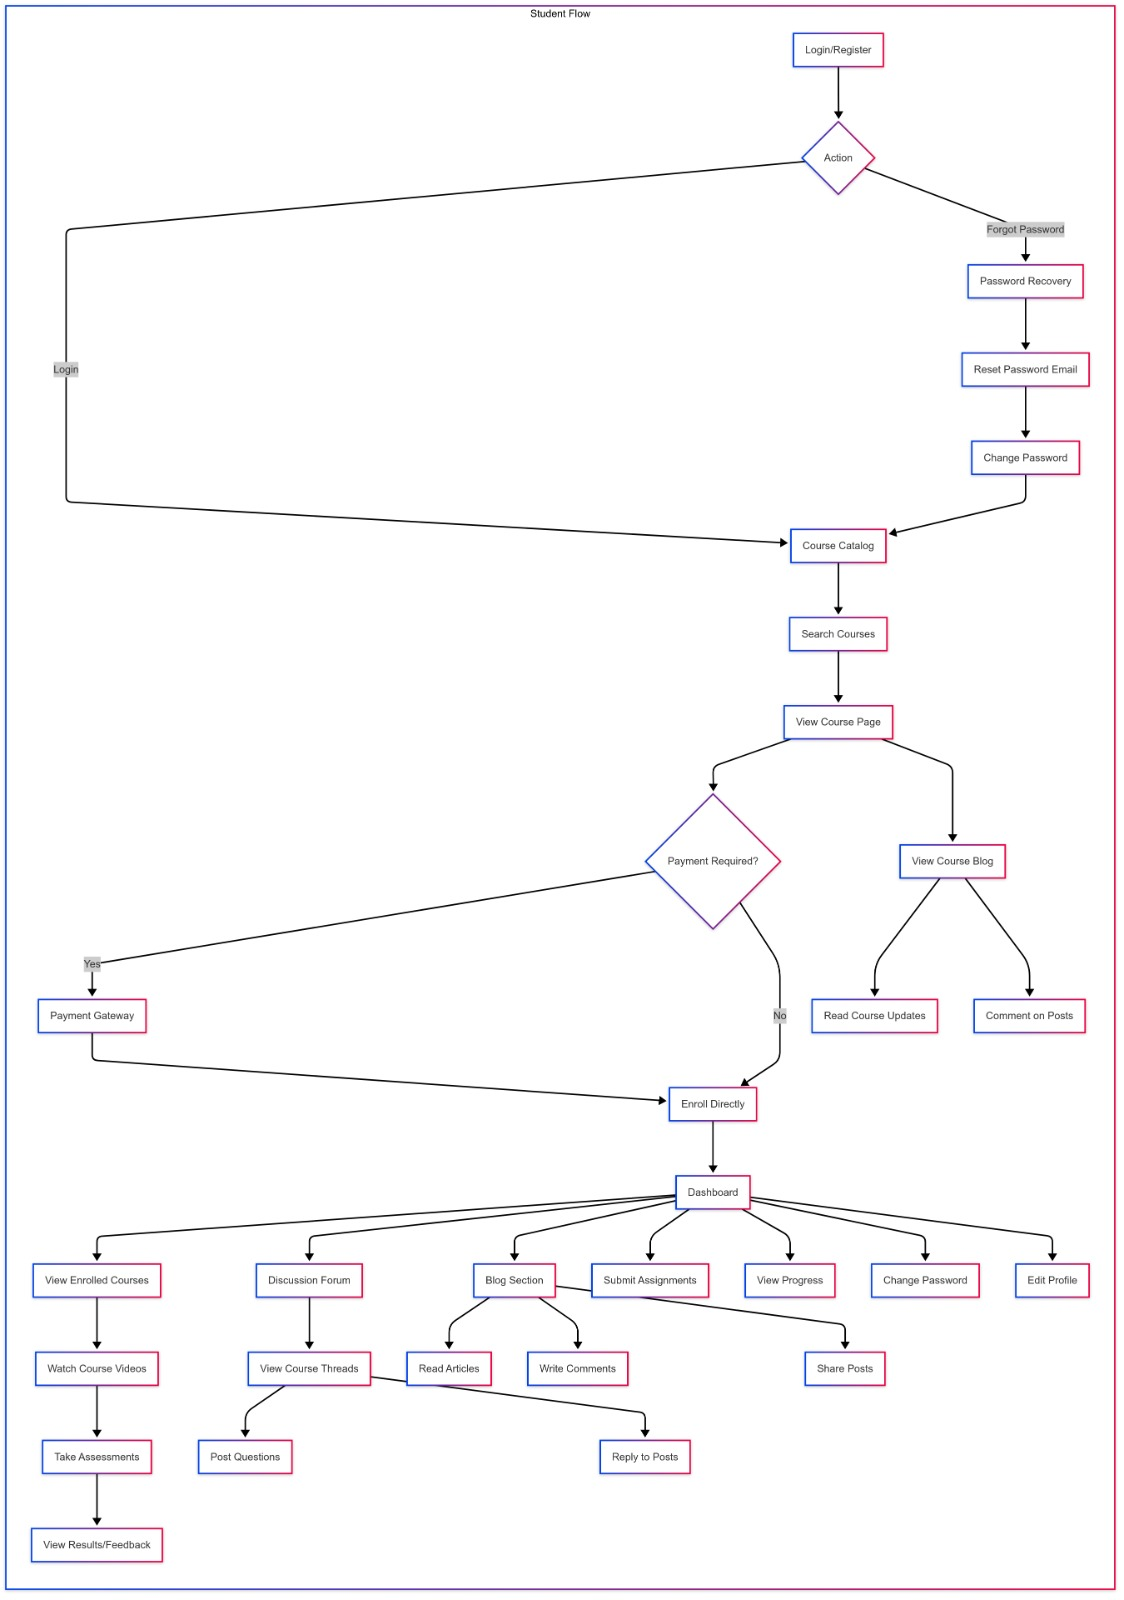
\includegraphics[height=0.63\textheight]{UI/stuFlow.jpg}
    \caption{Student Navigation Flow}
\end{figure}

\subsection{Educator}
\begin{figure}[!htb]
    \centering
    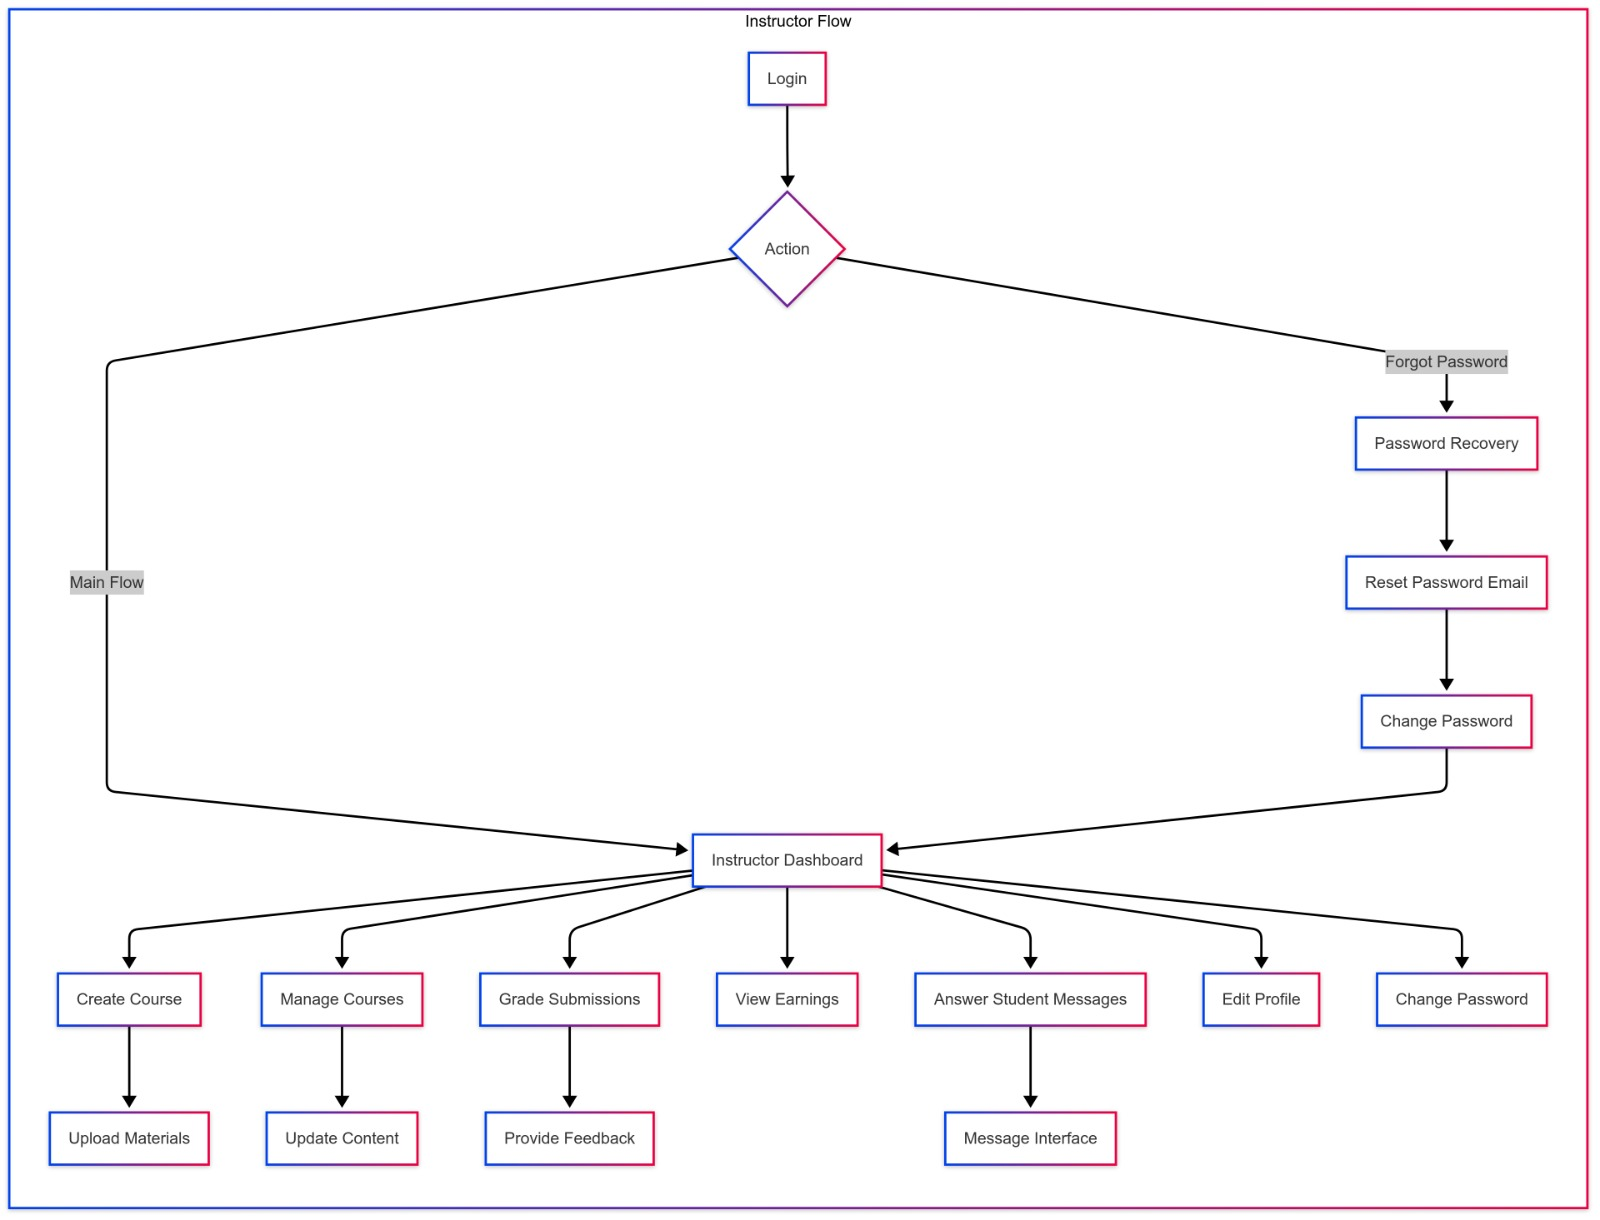
\includegraphics[height=0.3\textheight]{UI/eduFlow.jpg}
    \caption{Educator Navigation Flow}
\end{figure}

% Moderator and forum-related navigation removed

\section{Interface Storyboards}
\subsection{Authentication Flow}
\begin{figure}[ht]
    \centering
    \begin{subfigure}[b]{0.45\textwidth}
        \centering
        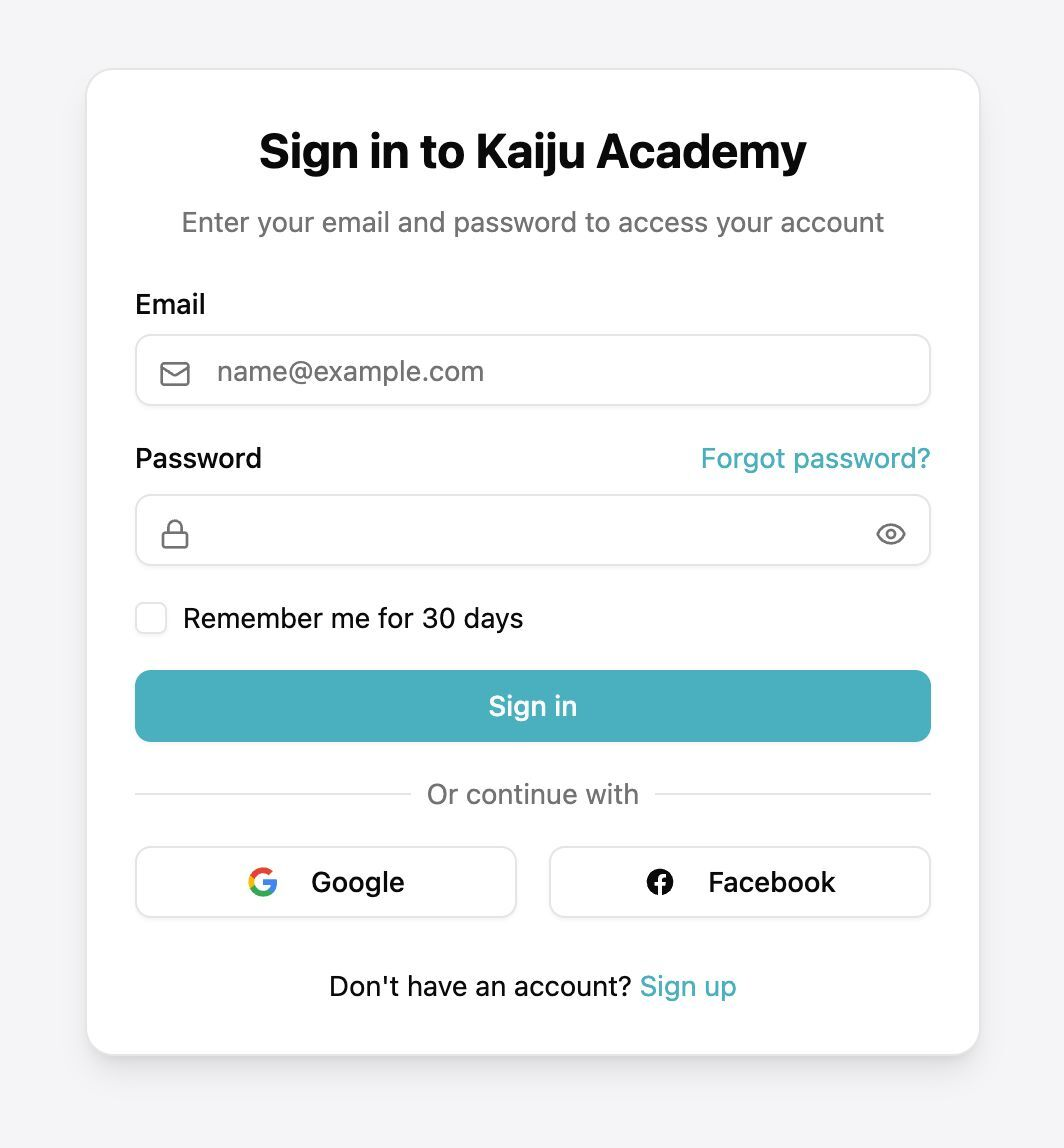
\includegraphics[width=\textwidth]{UI/SignIn.jpg}
        \caption{Sign In Screen}
    \end{subfigure}
    \hfill
    \begin{subfigure}[b]{0.45\textwidth}
        \centering
        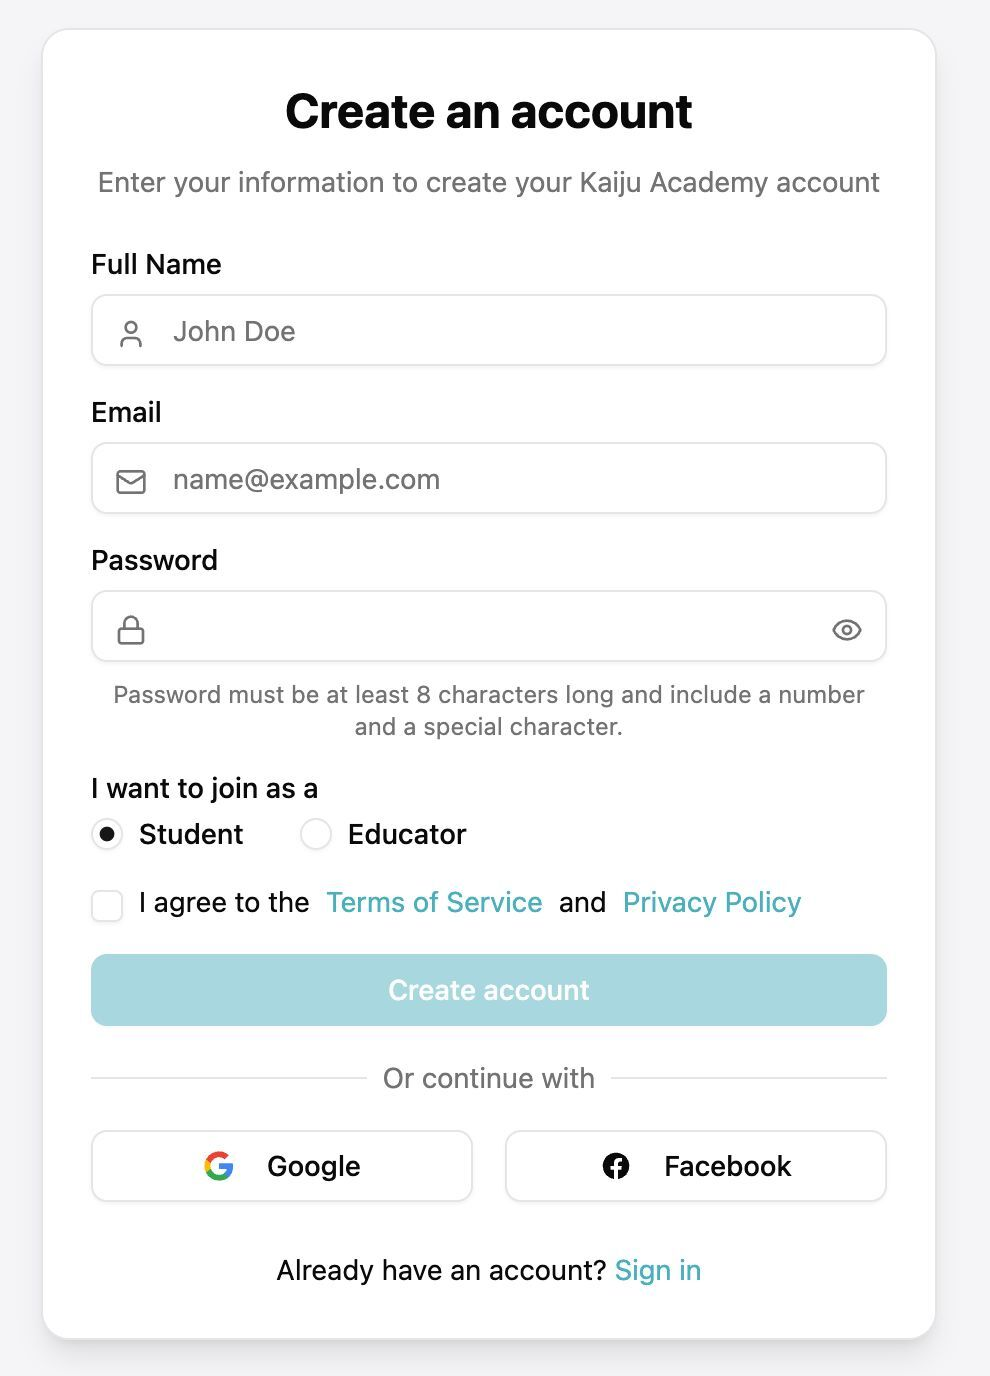
\includegraphics[width=\textwidth]{UI/SignUp.jpg}
        \caption{Sign Up Screen}
    \end{subfigure}
    \caption{Authentication Screens}
\end{figure}

\subsection{Student Learning Journey}
\begin{figure}[H]
    \centering
    \begin{subfigure}[b]{0.45\textwidth}
        \centering
        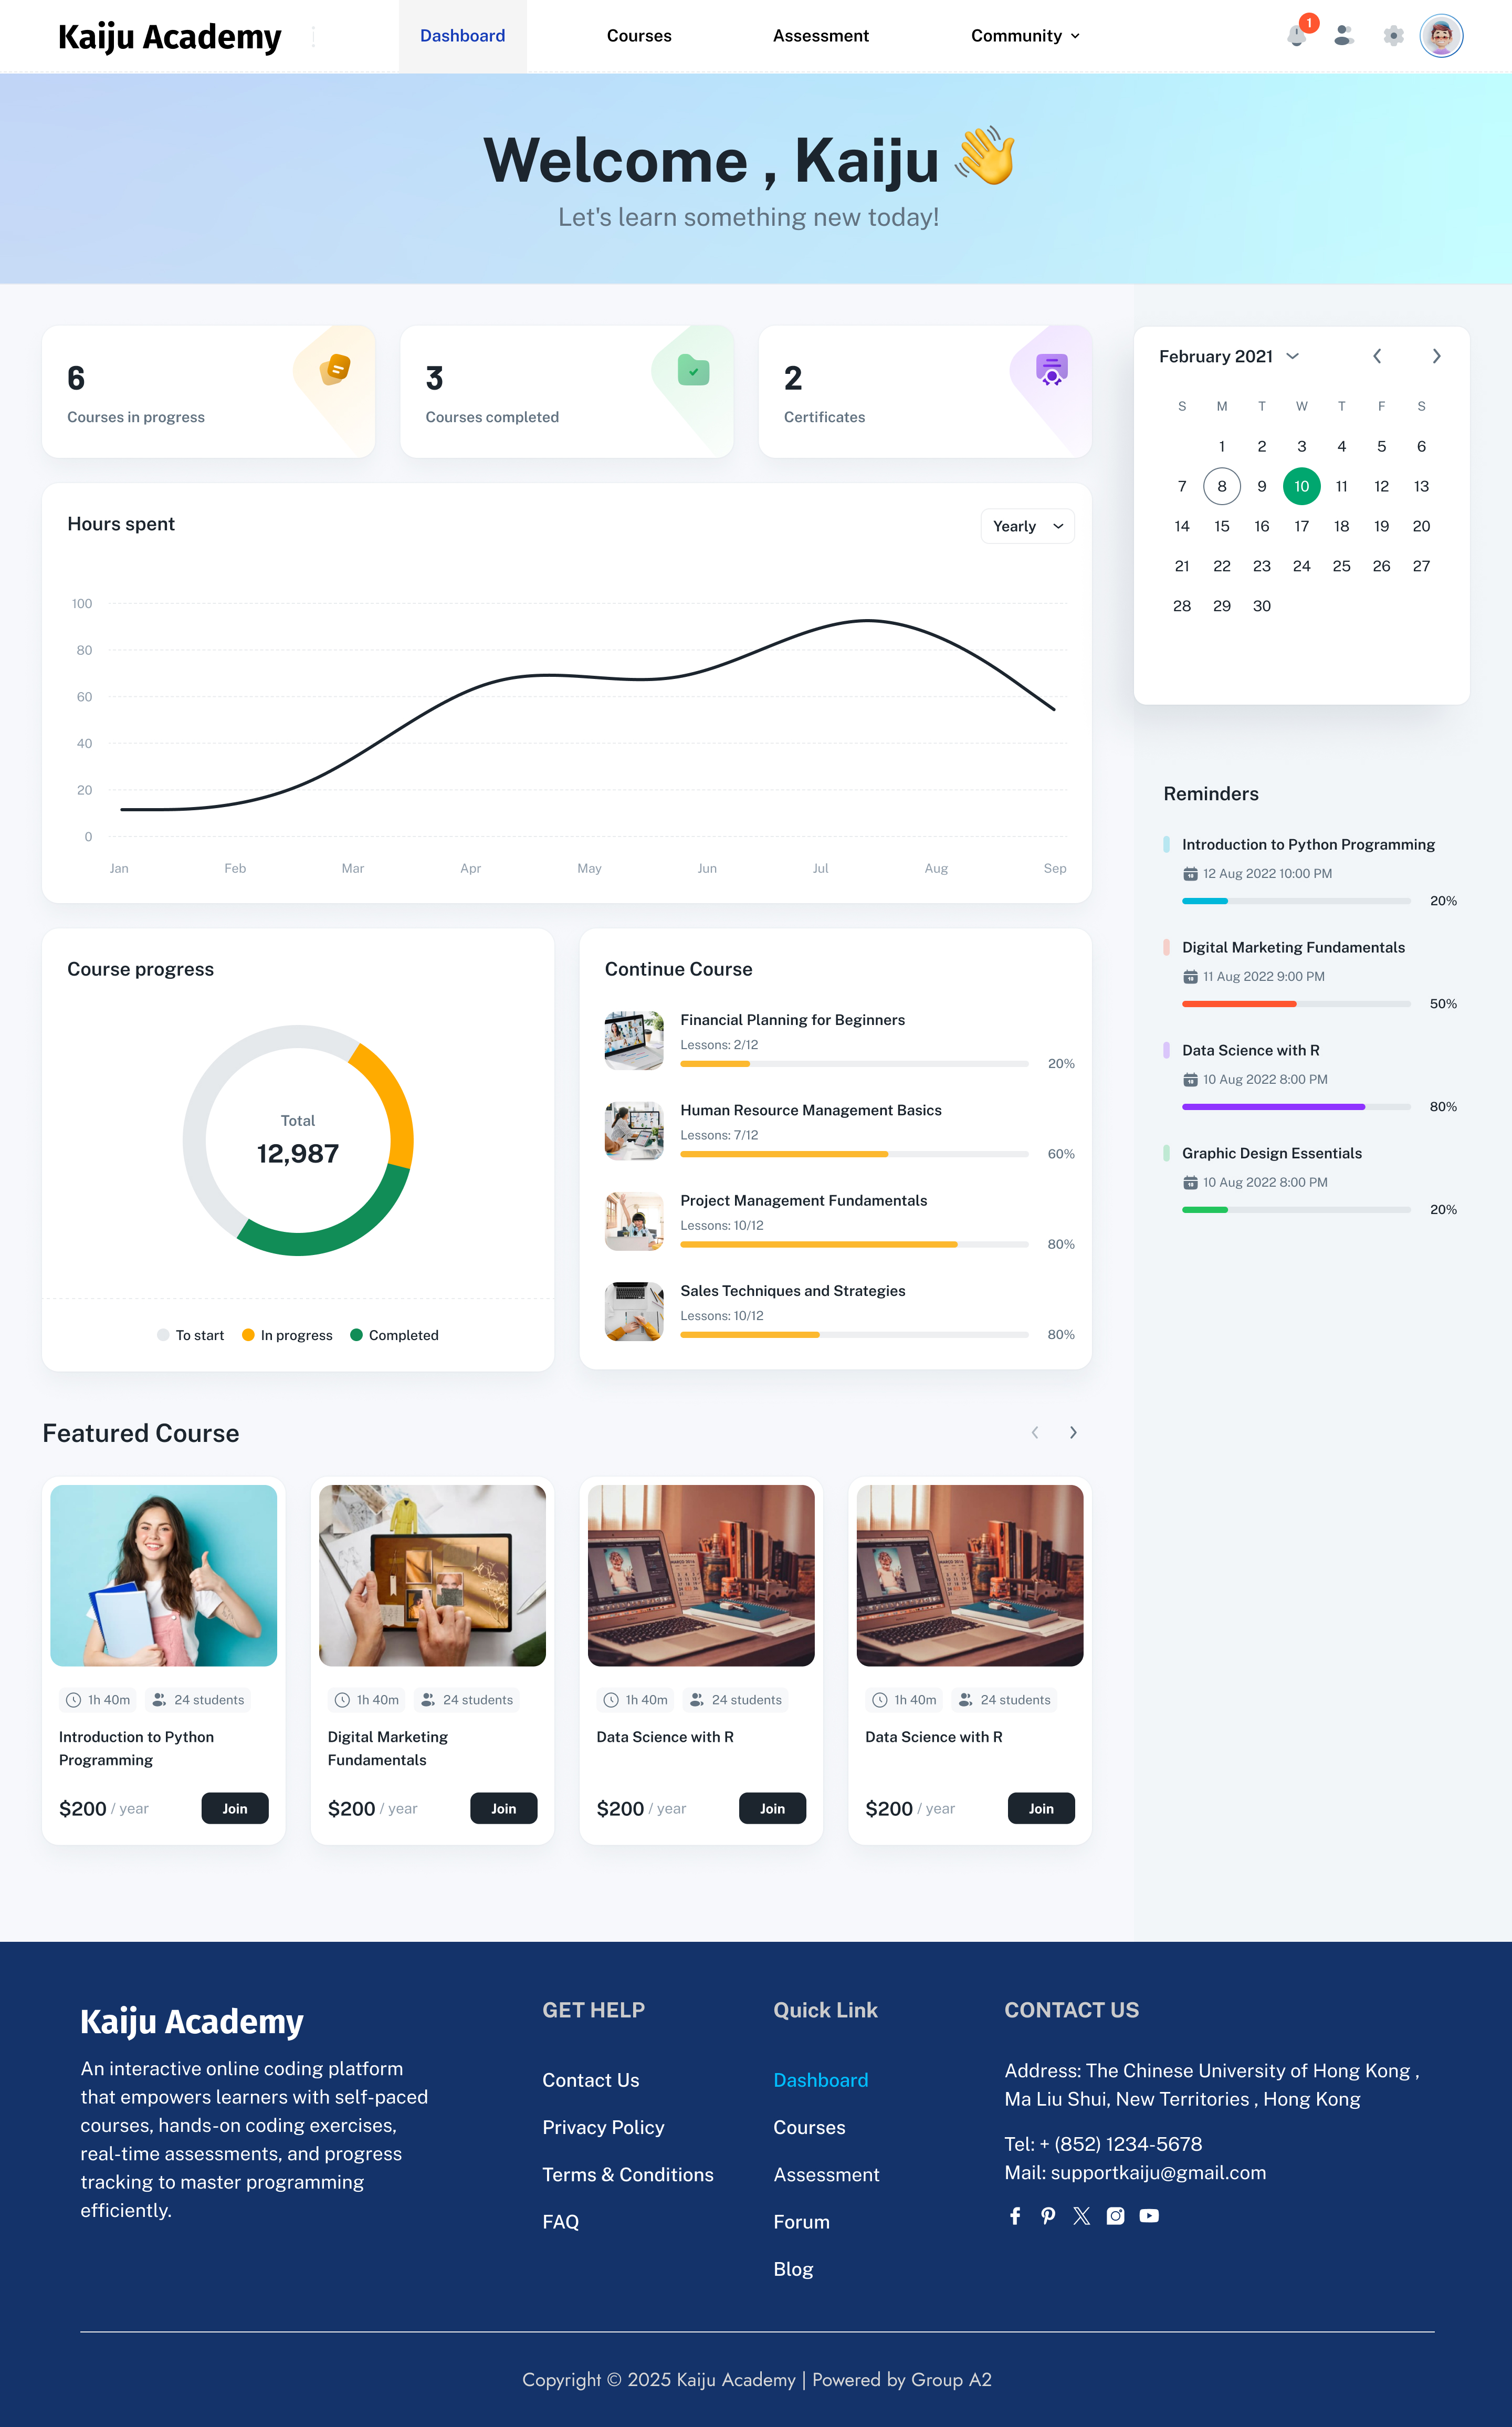
\includegraphics[height=0.4\textheight]{UI/Dashboard.jpg}
        \caption{Student Dashboard}
    \end{subfigure}
    \hfill
    \begin{subfigure}[b]{0.45\textwidth}
        \centering
        \includegraphics[height=0.4\textheight]{UI/All Courses.jpg}
        \caption{Course Catalog}
    \end{subfigure}
    \caption{Student courses view}
\end{figure}

\subsection{Learning Environment}
\begin{figure}[ht]
    \centering
    \begin{subfigure}[b]{0.47\textwidth}
        \centering
        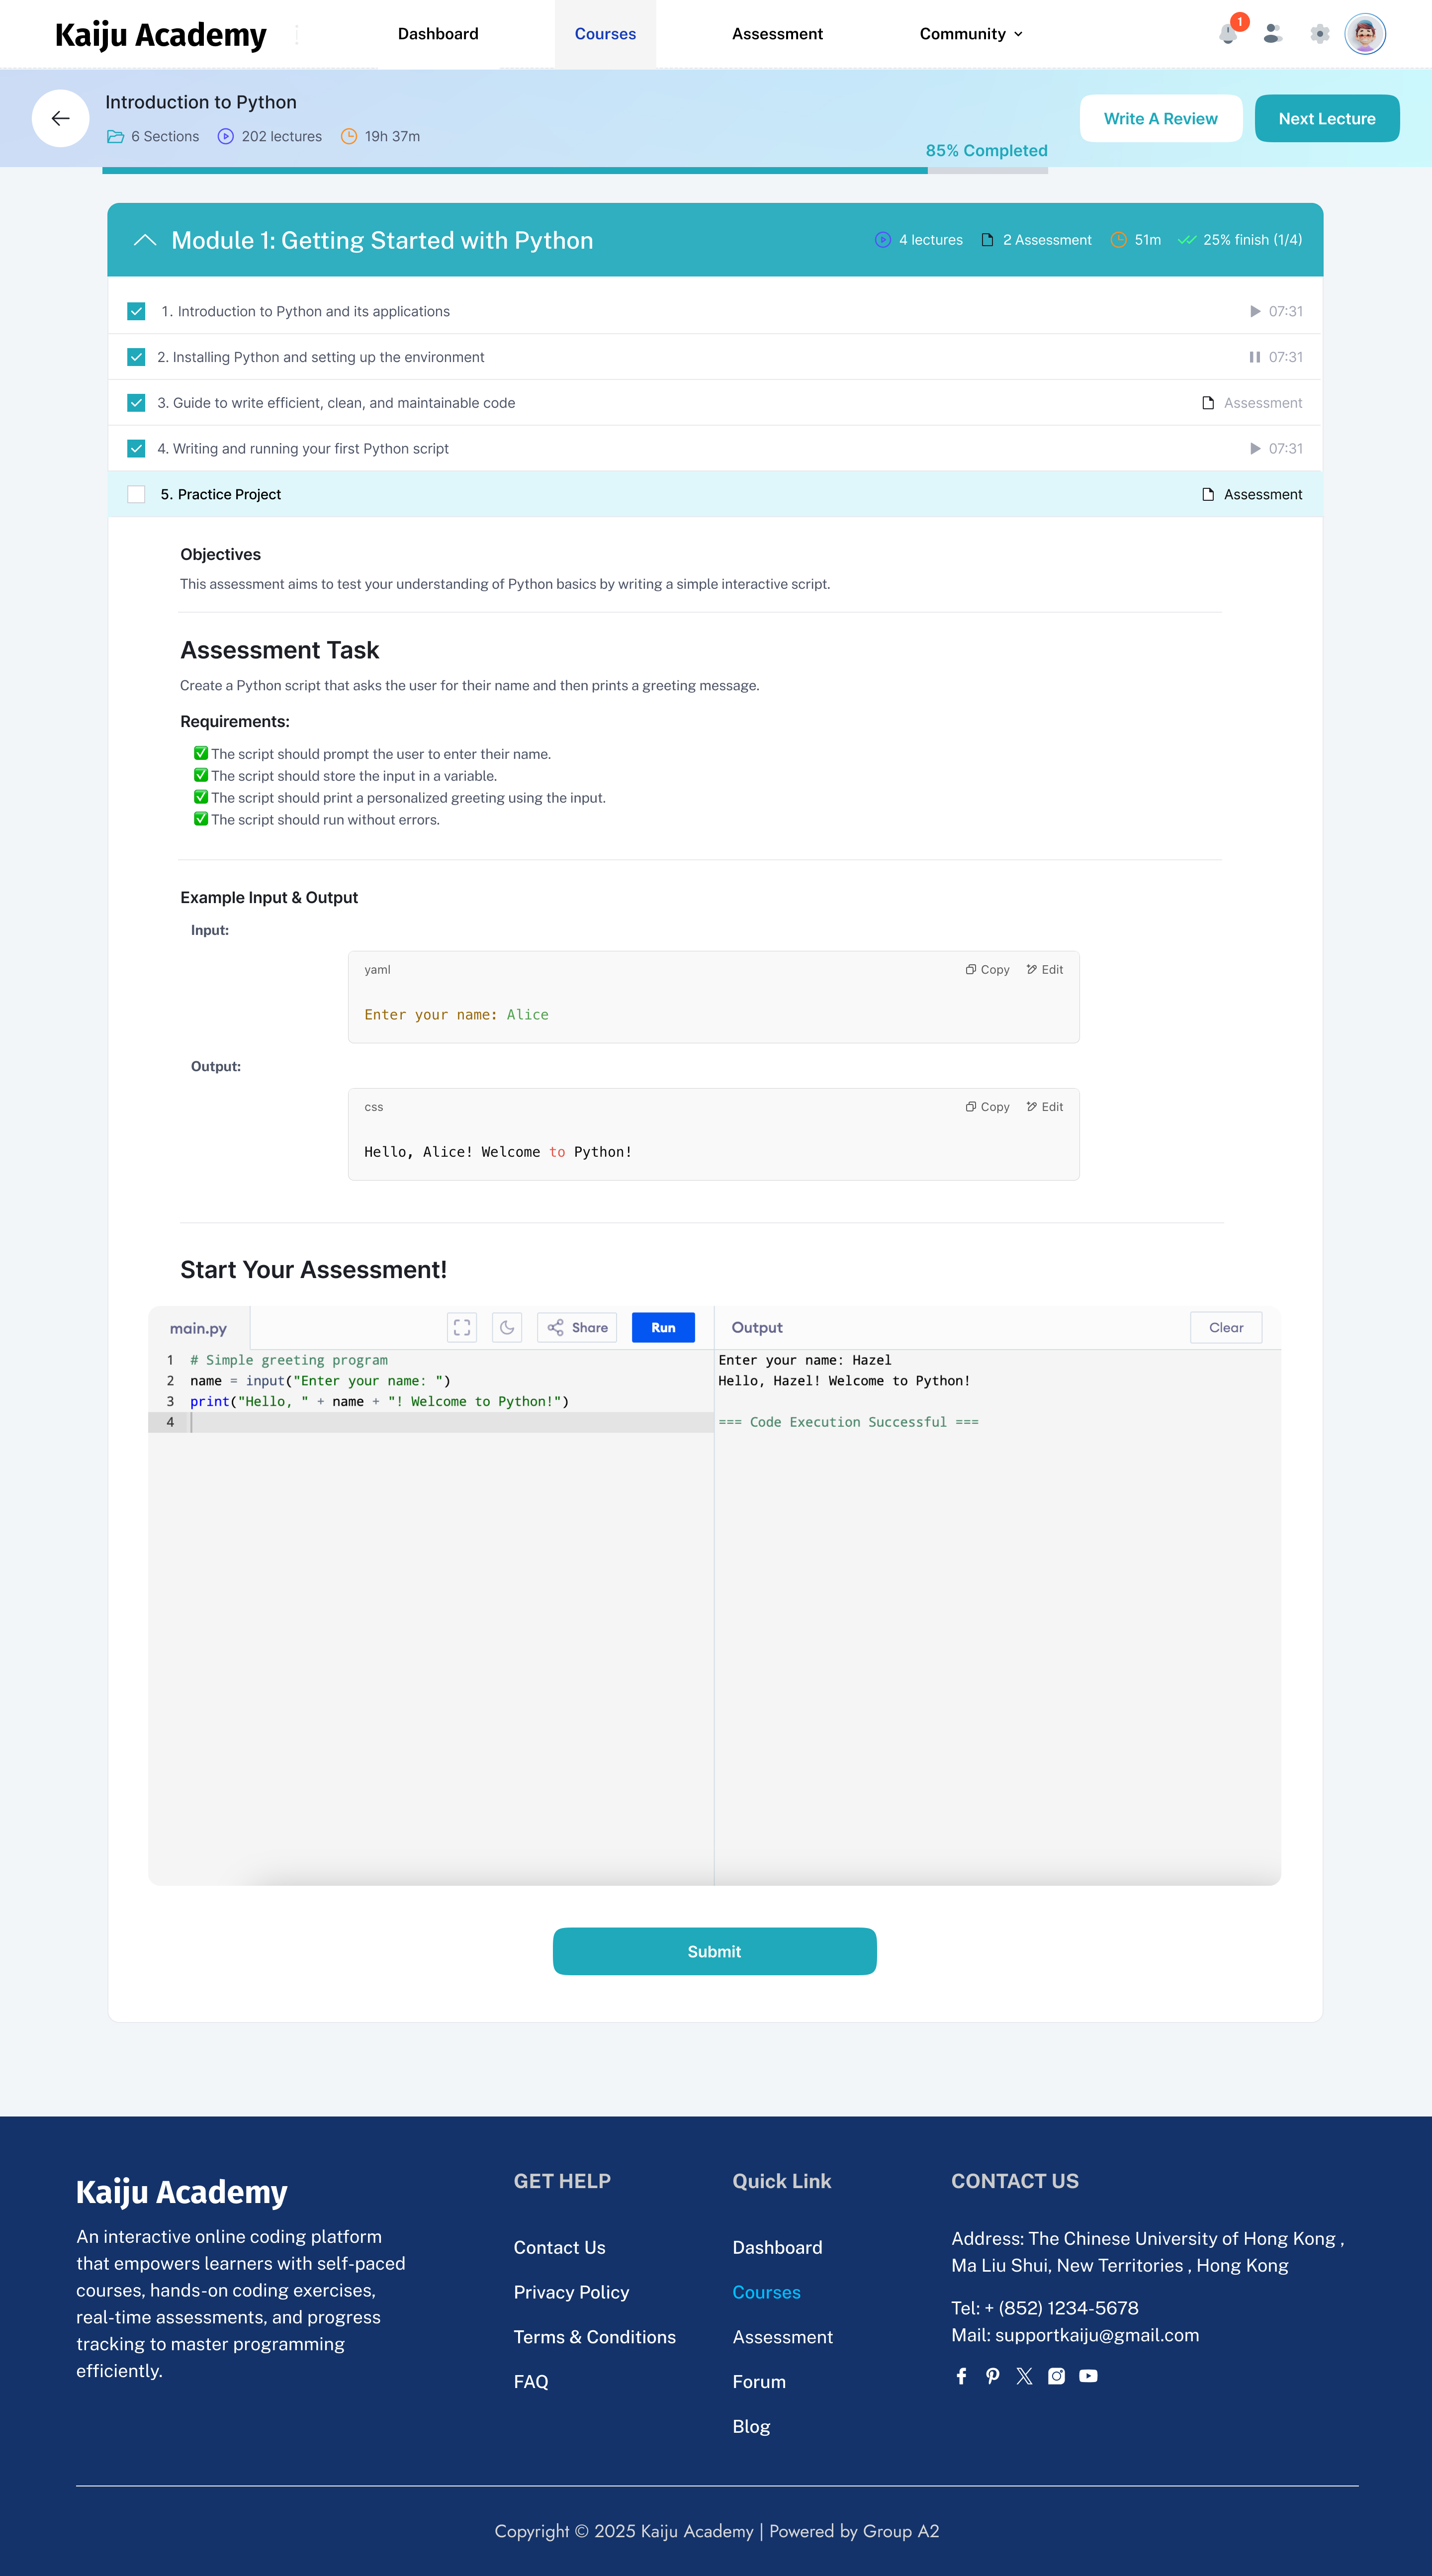
\includegraphics[width=\textwidth]{UI/Assessment.jpg}
        \caption{Assessment Interface}
    \end{subfigure}
    \hfill
    \begin{subfigure}[b]{0.47\textwidth}
        \centering
        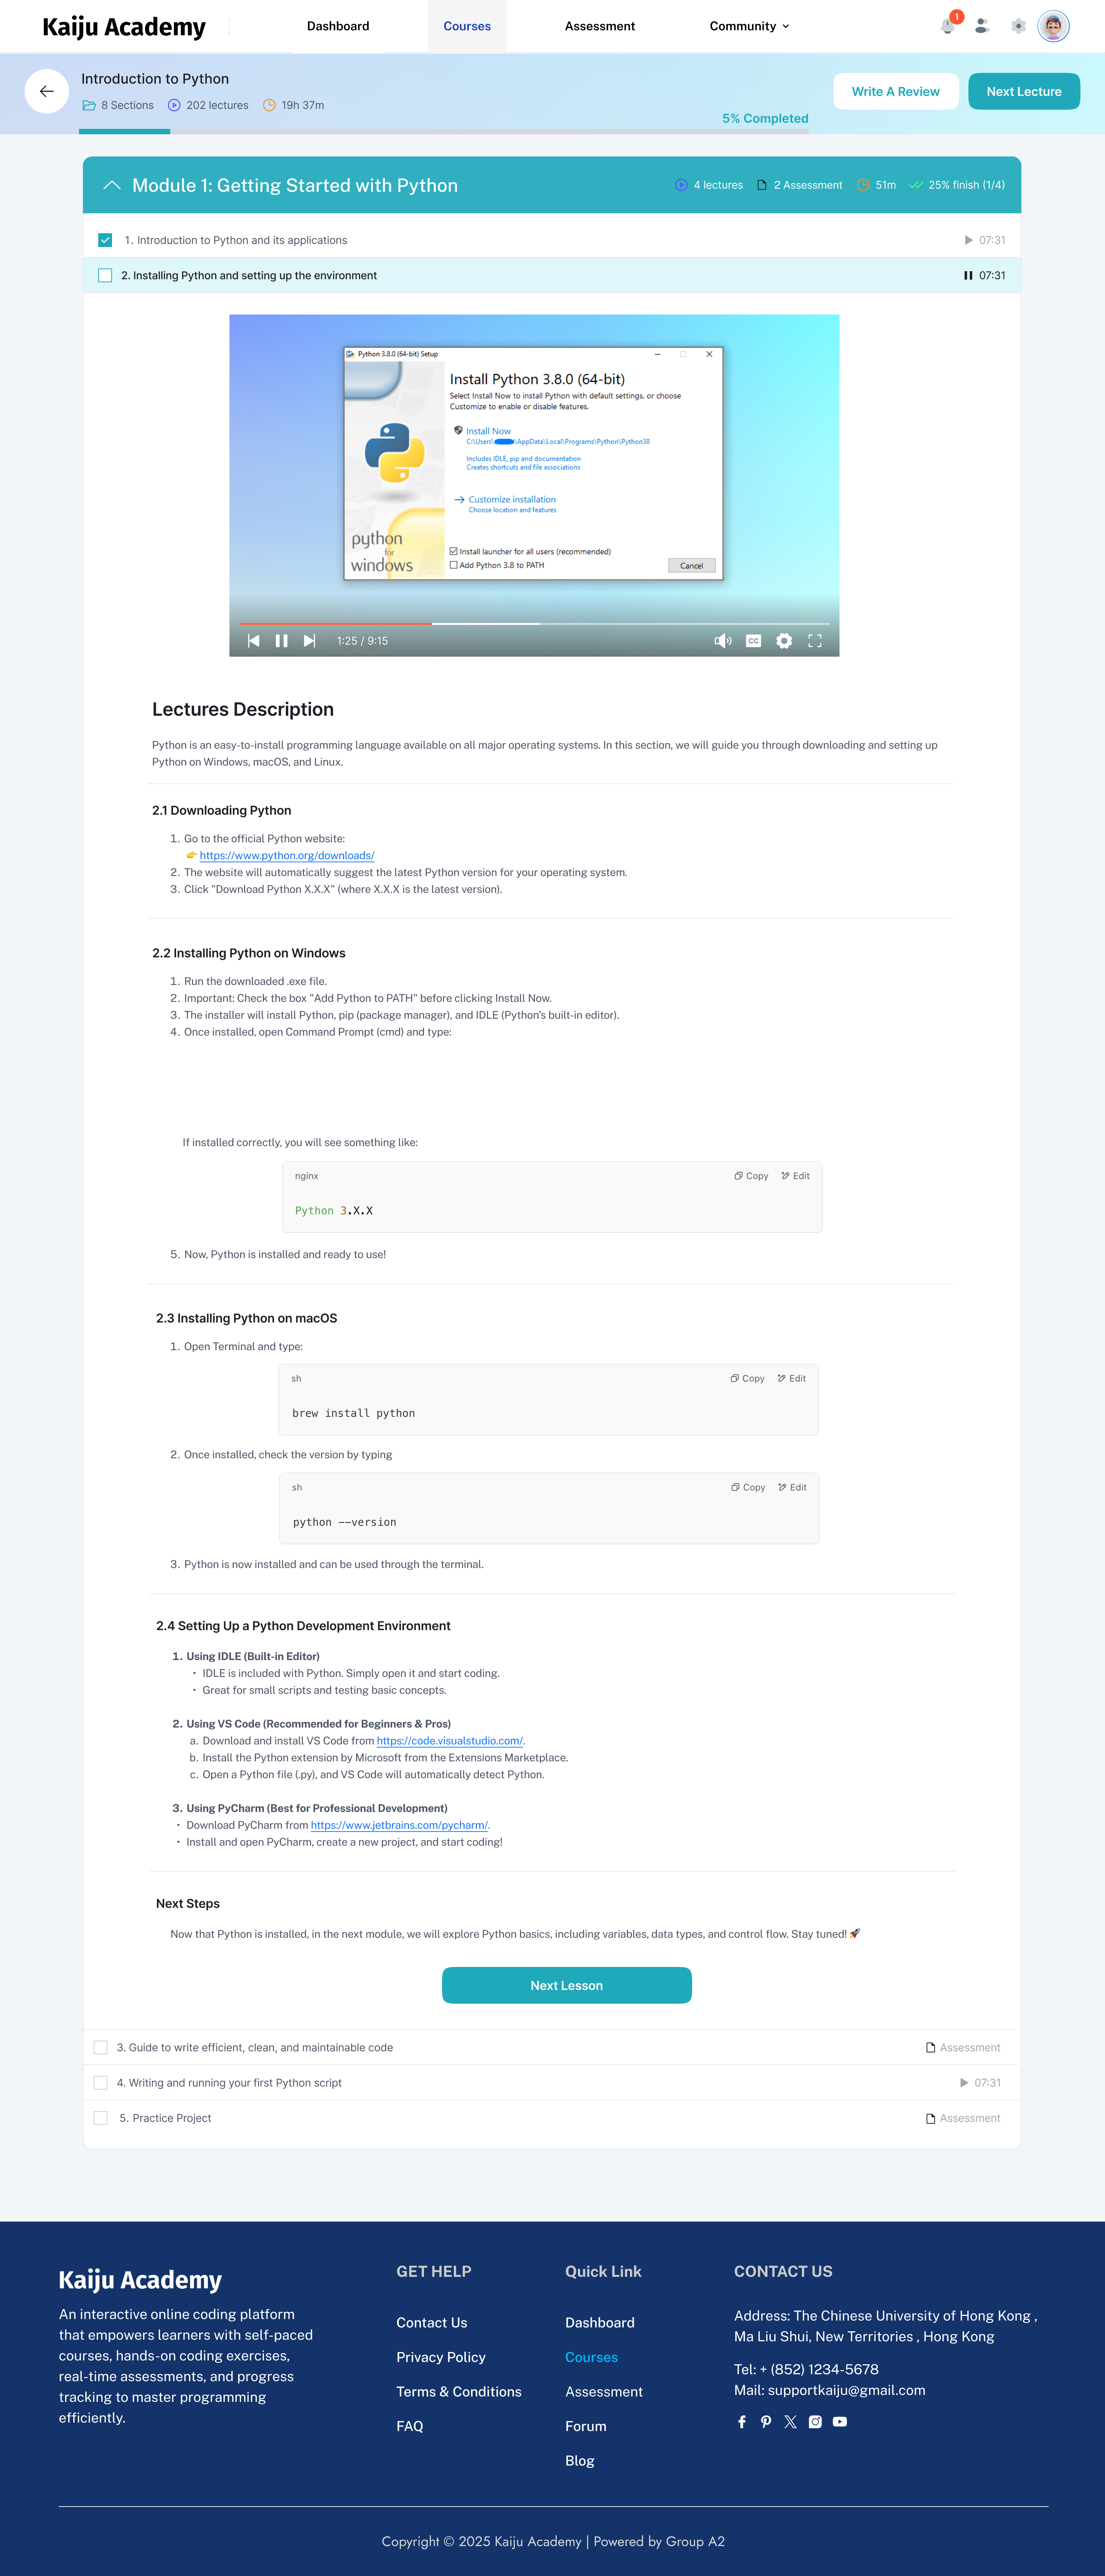
\includegraphics[width=\textwidth]{UI/During Course.jpg}
        \caption{During Course Interface}
    \end{subfigure}
    \caption{Learning and Assessment Interface}
\end{figure}

\section{Accessibility Considerations}
\begin{itemize}
    \item \textbf{Screen Reader Support:} Proper ARIA labels and semantic HTML
    \item \textbf{Text Resize:} Interface remains functional when text is enlarged 200\%
    \item \textbf{Motion Control:} Animations can be disabled
    \item \textbf{Alternative Text:} All images include descriptive alt text
    \item \textbf{Light/Dark Mode:} Option to switch between light and dark themes
    \item \textbf{Font Size Adjustment:} Users can easily change font size
\end{itemize}

\section{Responsive Design}
\begin{itemize}
    \item \textbf{Breakpoints:} 480px, 768px, 1024px, and 1440px
    \item \textbf{Layout:} 
    \begin{itemize}
        \item Single column on mobile
        \item Sidebar overlay on small screens
        \item Multi-column on larger screens
    \end{itemize}
    \item \textbf{Touch Targets:} Minimum 44$\times$44px for all interactives
\end{itemize}

\chapter{Assumptions}

\section{Technical Constraints}
\subsection{Hardware Constraints}
\begin{itemize}
    \item At least 4GB RAM, 320px width, 5 Mbps internet
    \item AWS cloud deployment, serverless Lambda, horizontal scaling
\end{itemize}

\subsection{Software Constraints}
\begin{itemize}
    \item Modern browsers (Chrome, Firefox, Safari, Edge, latest 2 versions)
    \item HTML5 and JavaScript required
    \item Responsive web (no native app initially)
\end{itemize}

\section{Operational Assumptions}
\begin{itemize}
    \item Peak: 10,000 code submissions/minute
    \item 80/20 read/write database
    \item Code execution max 5 seconds
    \item CI/CD pipeline with automated testing
    \item 99.9\% uptime excluding maintenance, daily backups
\end{itemize}

\section{Dependencies}
\subsection{Third-Party Services}
\begin{itemize}
    \item Authentication via OAuth providers (Google, GitHub, Microsoft)
    \item Payment processing for course credits
    \item Email delivery through Amazon SNS
    \item CDN via CloudFront
    \item Media transcoding via AWS MediaConvert
\end{itemize}

\end{document}